\documentclass{report}
\usepackage[utf8]{inputenc}
\usepackage{natbib}
\usepackage[dvipsnames]{xcolor}
\usepackage[pagestyles]{titlesec}
\usepackage[hidelinks]{hyperref}
\usepackage{pdfpages}
\usepackage{graphicx}
\usepackage{multicol}
\usepackage{multirow}
\usepackage{booktabs}
\usepackage{array}
\usepackage{tabularx}
\usepackage{ltablex}
\usepackage{listings}
\usepackage{alloy-style}

\newcolumntype{L}[1]{>{\raggedright\arraybackslash}p{#1}}
\newcolumntype{C}[1]{>{\centering\arraybackslash}p{#1}}
\newcolumntype{R}[1]{>{\raggedleft\arraybackslash}p{#1}}


\titleformat{\chapter}[display]{\normalfont\bfseries}{}{0pt}{\Huge}
\newpagestyle{mystyle}
{\sethead[\thepage][][\chaptertitle]{}{}{\thepage}}
\pagestyle{mystyle}

\begin{document}

\includepdf[pages={1}]{./img/FrontPage}
\tableofcontents
\chapter{Introduction}
This document represents the Requirement Analysis and Specification Document (RASD) for SafeStreets: an application that aims to improve the safety of urban areas by giving its users the possibility to report traffic violations to authorities. The goal of this document is to supply a description of the system in terms of its functional and non-functional requirements, listing all of its goals, discussing the constraints and the limits of the software, and indicating the typical use cases that will occur after the release. This document is addressed to the stakeholders, who will evaluate the correctness of the assumptions and decisions contained in it, and to the developers who will have to implement the requirements.
\section{Purpose}
SafeStreets is a crowd-sourced application that intends to provide users with the possibility to notify authorities when traffic violations occur. In order to report a traffic violation, users have to compile a report containing a picture of the violation, the date, time, position, and type of violation. SafeStreets stores all the information provided by users, completing it with suitable metadata (timestamps, sender's GPS position, etc.). In particular, in case the user had not provided any information regarding the license plate of the car breaking the traffic rules, SafeStreets runs an algorithm to read it from the submitted picture. Moreover, the application allows both citizens and authorities to check some useful statistics: in particular, SafeStreets is able to analyze the recieved information to build statistics and give suggestions to improve the safety of urban areas. If the municipality offers a service that allows users to retrieve the information about the accidents that occur in its territory, SafeStreets can cross this information with its own data.
Independently from Safestreets, the municipality could offer a service that takes the information about the violations coming from SafeStreets, and generates traffic tickets from it. In this case, SafeStreets ensures that the chain of custody of information coming from users is never broken, thus information is never altered. Information about issued tickets can be used by SafeStreets to build statistics, for example to have a feedback on the effectiveness of the application.
\subsection{Goals}
\begin{itemize}
    \item {[G.1]} Allow the Users to access the functionalities of the application from different locations and devices.
	\item {[G.2]} Allow Guests to authenticate either as Authority or Citizen.
    \item {[G.3]} Allow the User to document traffic violations and accidents by compiling a Report.
    \item {[G.4]} Store the reports provided by the Citizens.
    \begin{itemize}
    		\item {[G.4.1]} If the Citizen has not provided any information about the license plate, the System runs an algorithm to read it from the submitted picture.
		\end{itemize}     
	\item {[G.5]} Allow Authorities to consult the reports submitted by the Citizens.
    \item {[G.6]} Analyze the stored information to build statistics.
    \begin{itemize}
    		\item {[G.6.1]}If allowed by the Municiplaity, SafeStreets can cross their information about accidents with its own in order to improve the analysis.
	\end{itemize}  
	\item {[G.7]} Detect unsafe areas through statistics.
	\begin{itemize}
		\item {[G.7.1]}Suggest possible interventions to the Authorities.
	\end{itemize}
	\item{[G.8]}Build statistics on iussued tickets if the Municiplaity allows SafeStreets to access such data.
    \begin{itemize}
        \item {[G.8.1]} Ensure that the chain of custody of the information coming from the Citizens is never broken.
	\end{itemize}
	\item {[G.9]} Allow the Users to consult statistics.
	\begin{itemize}
		\item {[G.9.1]} Offer different levels of visibility to different roles.
	\end{itemize}
\end{itemize}

\section{Scope}
According to the \textit{World} and \textit{Machine} paradigm, proposed by M. Jackson and P. Zave in 1995, we can distinguish the \textit{Machine}, that is the portion of the system to be developed, from the \textit{World}, that is the portion of the real-world affected by the machine. In this way, we can classify the phenomena in three different types: World, Machine and \textit{Shared} phenomena, where the latter type of phenomena can be controlled by the world and observed by the machine or controlled by the machine and observed by the world:
\newline
In this context, the most relevant phenomena are organized as in the following table.

\begin{table}[p]
		%{pix.acc.} & {mean.acc.} & {mean.IoU} & {f.w.IoU}
		\begin{center}
		%\hspace{-4.5cm}
		\begin{tabular}{|C{.28\textwidth}||C{.28\textwidth}||C{.28\textwidth}|}
			\toprule
			\textbf{World} &\textbf{Shared}& \textbf{Machine}\\
			\midrule
			\midrule
			\textbf{Traffic violation}: circumstance in which someone doesn't respect the traffic rules &\textbf{\small{Registration/Login}}$^{1}$: a Guest can sign up to the application or log in if already registered.&\textbf{DBMS query}: operation performed to retrieve/store data\\
			\midrule
			\textbf{Accident}: event that caused damage to things or people.&\textbf{Commit of a report}$^{1}$: action of sending a report documenting a traffic violation or an accident.&\textbf{API queries}: request for third-part services.\\
			\midrule
			&\textbf{Send notifications}$^{2}$: to notify the Authorities when a report is submitted.&\textbf{Encrypt data}: to compute the hash function to ensure that reports are never altered and that user's credentials are safe.\\
			\midrule
			&\textbf{Build statistics}$^{2}$: computation of statistics to find unsafe areas, to see which veichles commit multiple infractions and also to monitor the trend of issued tickets.&\textbf{Role Isolation}: to grant different levels of visibility to Citizen and Authorities\\ 
			\midrule			
			&\textbf{Safety Suggestionss}$^{2}$: to give suggestions for possible safe interventions (e.g add a barrier).&\\
			\bottomrule
		\end{tabular}
		\end{center}
		\caption{In the table above, \textit{1} refers to shared phenomena controlled by the world and observed by the machine, whereas \textit{2} refers to the phenomena controlled by the machine and observed by the world}.
		\label{tab:multicol}
	\end{table}
\clearpage
\section{Definitions, Acronyms and Abbreviations}
\subsection{Definitions}
\begin{itemize}
	\item \textit{System}: the totality of the hardware/software applications that contribute to provide the service concerned.
    \item \textit{Guest}: someone who has yet to sign up and who is not able to access any feature of the application.
    \item \textit{User}: a registered user who has logged in.
	\begin{itemize}
		\item \textit{Citizen}: user who can send Reports of traffic violation. It has limited visibility over the stored information.
		\item \textit{Authority}: user who has access to the history of Reports and is notified whenever a new Report is recieved. It has full visibility over the data exposed by the System.
	\end{itemize} 
	\item \textit{Municipality}: a single administrative division with its own local government. It stores sensitive information about the Authorities and their work (g.e. traffic tickets).
    \item \textit{Traffic violation}: occurrence of drivers that violate laws that regulate vehicle operation on streets and highways(e.g double-way parking).
    \item \textit{Safety Suggestion}: recommendation to improve the safety of urban areas. It is computed by analyzing the statistics built by the system.
    \item \textit{Report}: documentation of a traffic violation. It contains a picture of the violation, the date, time, position, and type of violation. Some fields can be omitted in case an accident is being reported.
    \item \textit{Hash}: a mathematical algorithm that maps data of arbitrary size to a bit string of fixed size. It is a one-way function, that is, a function which is practically infeasible to invert.
    \item \textit{Chain of custody}: chronological documentation that records the sequence of custody, control, transfer, analysis, and disposition of physical or electronic evidence.
    \item \textit{Third-party services}: services used by the System in order to provide extra functionalities (e.g. image recognition).
\end{itemize}
\subsection{Acronyms}
\begin{itemize}
\item \textbf{API}: \textit{Application Program Interface}, set of routines, protocols and tools for building software applications on top of this one.
\item \textbf{OCR}: \textit{Optical Character Recognition}, software dedicated to the detection of characters contained in a document and to their transfer to digital text that can be read by a machine. In this context, OCR will be used to read license plates.
\item \textbf{UML}: \textit{Unified Modeling Language}, is a standard visual modeling language intended to be used for analysis, design, and implementation of software-based systems.
\item \textbf{GPS}: \textit{Global Positioning System}, technology widely used to get the user's position.
\item \textbf{DBMS}: \textit{Data Base Management System}, software that provides organized space memory to store information.
\item \textbf{ID}: \textit{Identification}, a unique key given to each registered User.
\end{itemize}
\subsection{Abbreviations}
\begin{itemize}
\item {[G$_{i}$]}: i-th goal.
\item {[R$_{i}$]}: i-th requirement.
\item {[D$_{i}$]}: i-th domain assumption.
\end{itemize}
\section{Reference Documents} \label{docs}
\begin{itemize}
	\item Specification document: \textit{SafeStreets Mandatory Project Assignment.pdf}.
	\item IEEE std 830-1998:  \href{http://www.math.uaa.alaska.edu/~afkjm/cs401/}{\textit{IEEE Recommended Practice for Software Requirements Specifications}}.
	\item ISO/IEC 9126-1:2001: \href{https://www.iso.org/standard/22749.html}{\textit{Software engineering — Product quality — Part 1: Quality model}}
	\item Alloy docs: \url{http://alloy.lcs.mit.edu/alloy/documentation.html}.
	\item UML diagrams: \url{https://www.uml-diagrams.org}.
\end{itemize}
\section{Document Structure}
This document is presented as it follows:
\begin{enumerate}
	\item {\textbf{Introduction}} contains a general description of the system and its goals, presenting the problem in an informal way.
	\item{\textbf{Overall description}} gives a general description of the application, focusing on the context of the system and giving further details about shared phenomena. Furthermore, we will provide the specifications of constraints, dependencies and assumptions, that show how the System is integrated with the real world.
	\item{\textbf{Specific requirements}} goes into details about functional and non functional requirements and a list of all possible interctions with the System is provided using use cases and sequence diagrams.
	\item {\textbf{Formal analysis using Alloy}} contains the Alloy model of some critical aspects of the System with all the related comments. A proof of consistency and an example of the generated world are also provided.
	\item {\textbf{Effort spent}} shows the time spent writing this document by each member of the team.
\end{enumerate}

\chapter{Overall Description}
\section{Product Perspective}
We are going to analyze all the shared phenomena that are listed in the previous section. The concepts are clarified through class and state diagrams.\\ \vspace{2mm}

\noindent\textbf{Registration/Login} (World controlled, Machine observed)\\
A Guest can sign up to the application or log in, if already registered. 
In the case of a new submit, the System provides a form which the Guest have to fill with his data, specifying if he/she is 
a Citizien or an Authority.\\ \vspace{2mm}

\noindent\textbf{Commit of a report} (World controlled, Machine observed)\\
A Citizen can send a Report with a description of the violation compiling a structured field. He/she has the possibility to  attach a picture. The System will check if the compiled fields are consistent and complete, then it will encrypt the Report and send it to the Storage Manager (Figure \ref{fig:State1}). \\ \vspace{2mm}

\noindent\textbf{Send Notification} (Machine controlled, World observed)\\
The System notifies the Authorities whenever a new Report is submitted by a Citizen. 
We assume that the notified Authorities will accordingly handle the violation reported. (Figure \ref{fig:State1}).
\begin{figure}[!ht]
\begin{center}
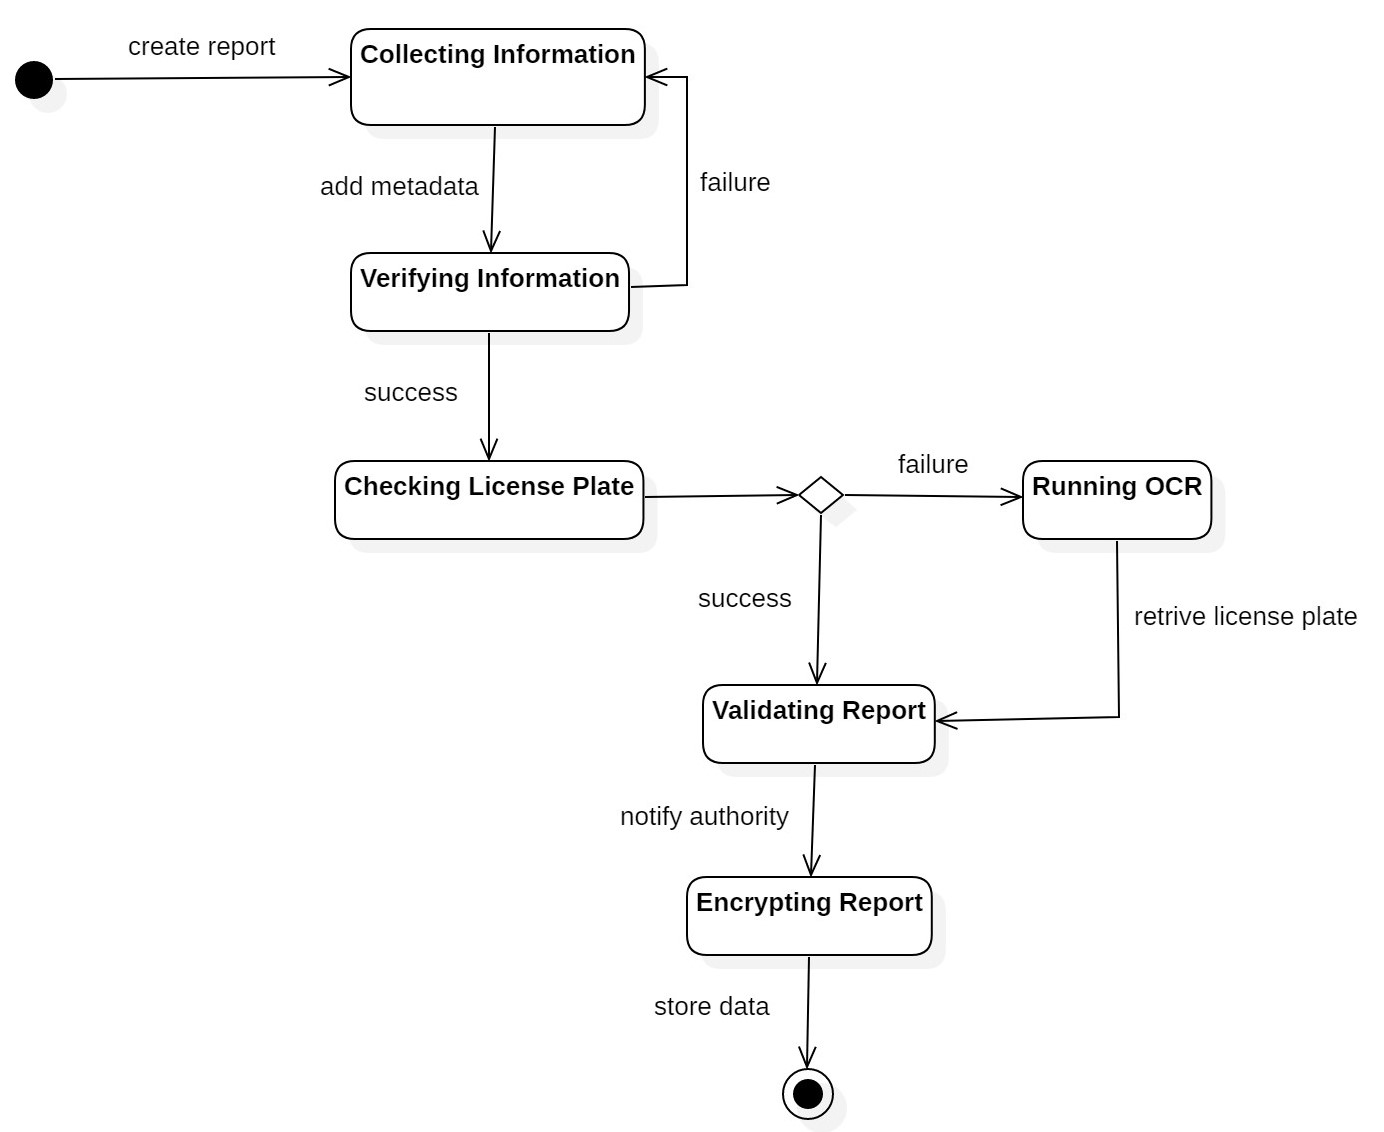
\includegraphics[width=.8\textwidth]{./img/Statechart_Report.jpg}
\end{center}
\caption{SafeStreets' statechart diagram about the collection, notification, and storage of a Report.}
\label{fig:State1}
\end{figure} 
\newpage
\noindent\textbf{Build statistics} (Machine controlled, World observed)\\
The System analyzes the stored data and computes general statistics on the violations. In this way, the System is able to find unsafe areas and which vehicles commit the most violations. All Users can access general statistics, however only Authorities can request statistics on private information such as traffic tickets. If the System is allowed to access Municipality's data, statistics can be enhanced by crossing it with SafeStreets' information (Figure \ref{fig:State2}).  \\ \vspace{2mm}

\noindent\textbf{Safety Suggestionss} (Machine controlled, World observed)\\
The System gives Authorities suggestions for possible safe interventions. His knowledge is based on the statistics previously computed (Figure \ref{fig:State2}).

\begin{figure}[!ht]
\begin{center}
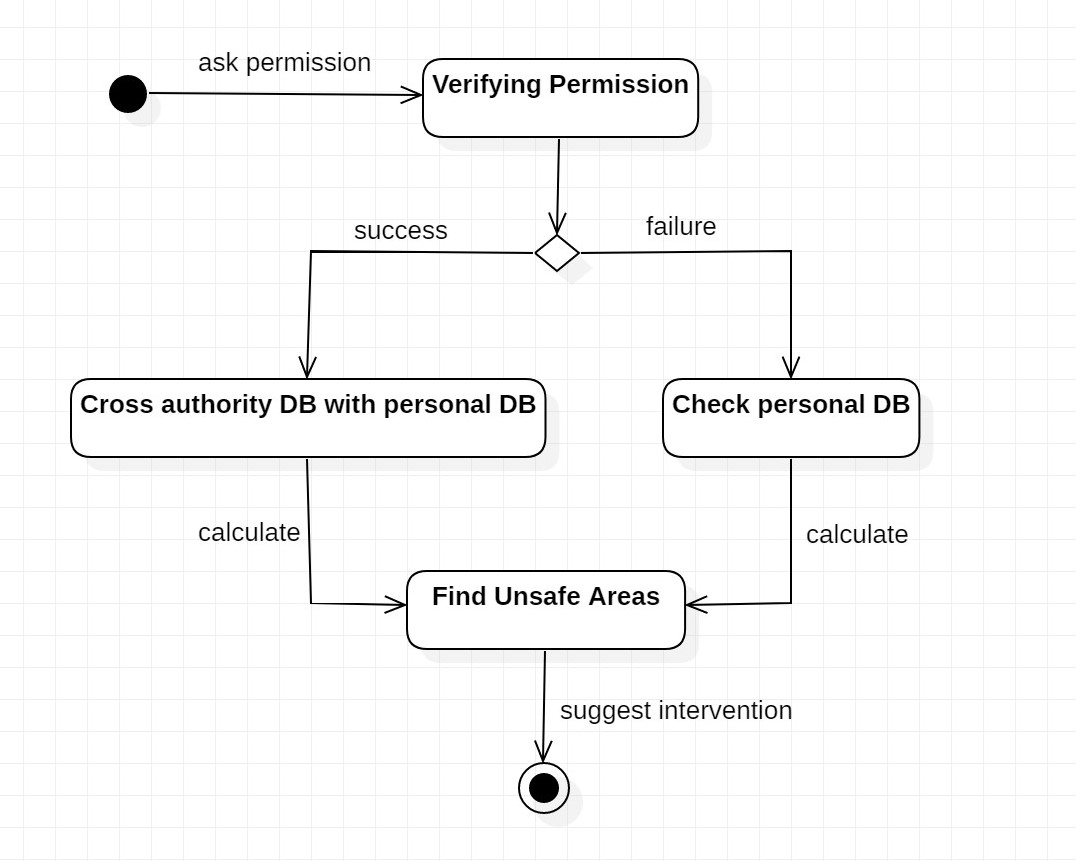
\includegraphics[width=.8\textwidth]{./img/img_UnsafeAreas.jpg}
\end{center}
\caption{SafeStreets' statechart diagram of the creation of statistics on unsafe areas.}
\label{fig:State2}
\end{figure}
\newpage
\subsection{Class Diagram}
The class diagram in Figure \ref{fig:UML} shows a possible representation of the Safe Streets' architecture. Notice that the Municipality's database is only accessible by the System if SafeStreets is authorized by the Municipality Manager. It's also important to outline that the System is not designed to provide a function to generate official traffic tickets, since only real world authorities (g.e. local police) can generate traffic tickets with legal validity.
\begin{figure}[!ht]
\begin{center}
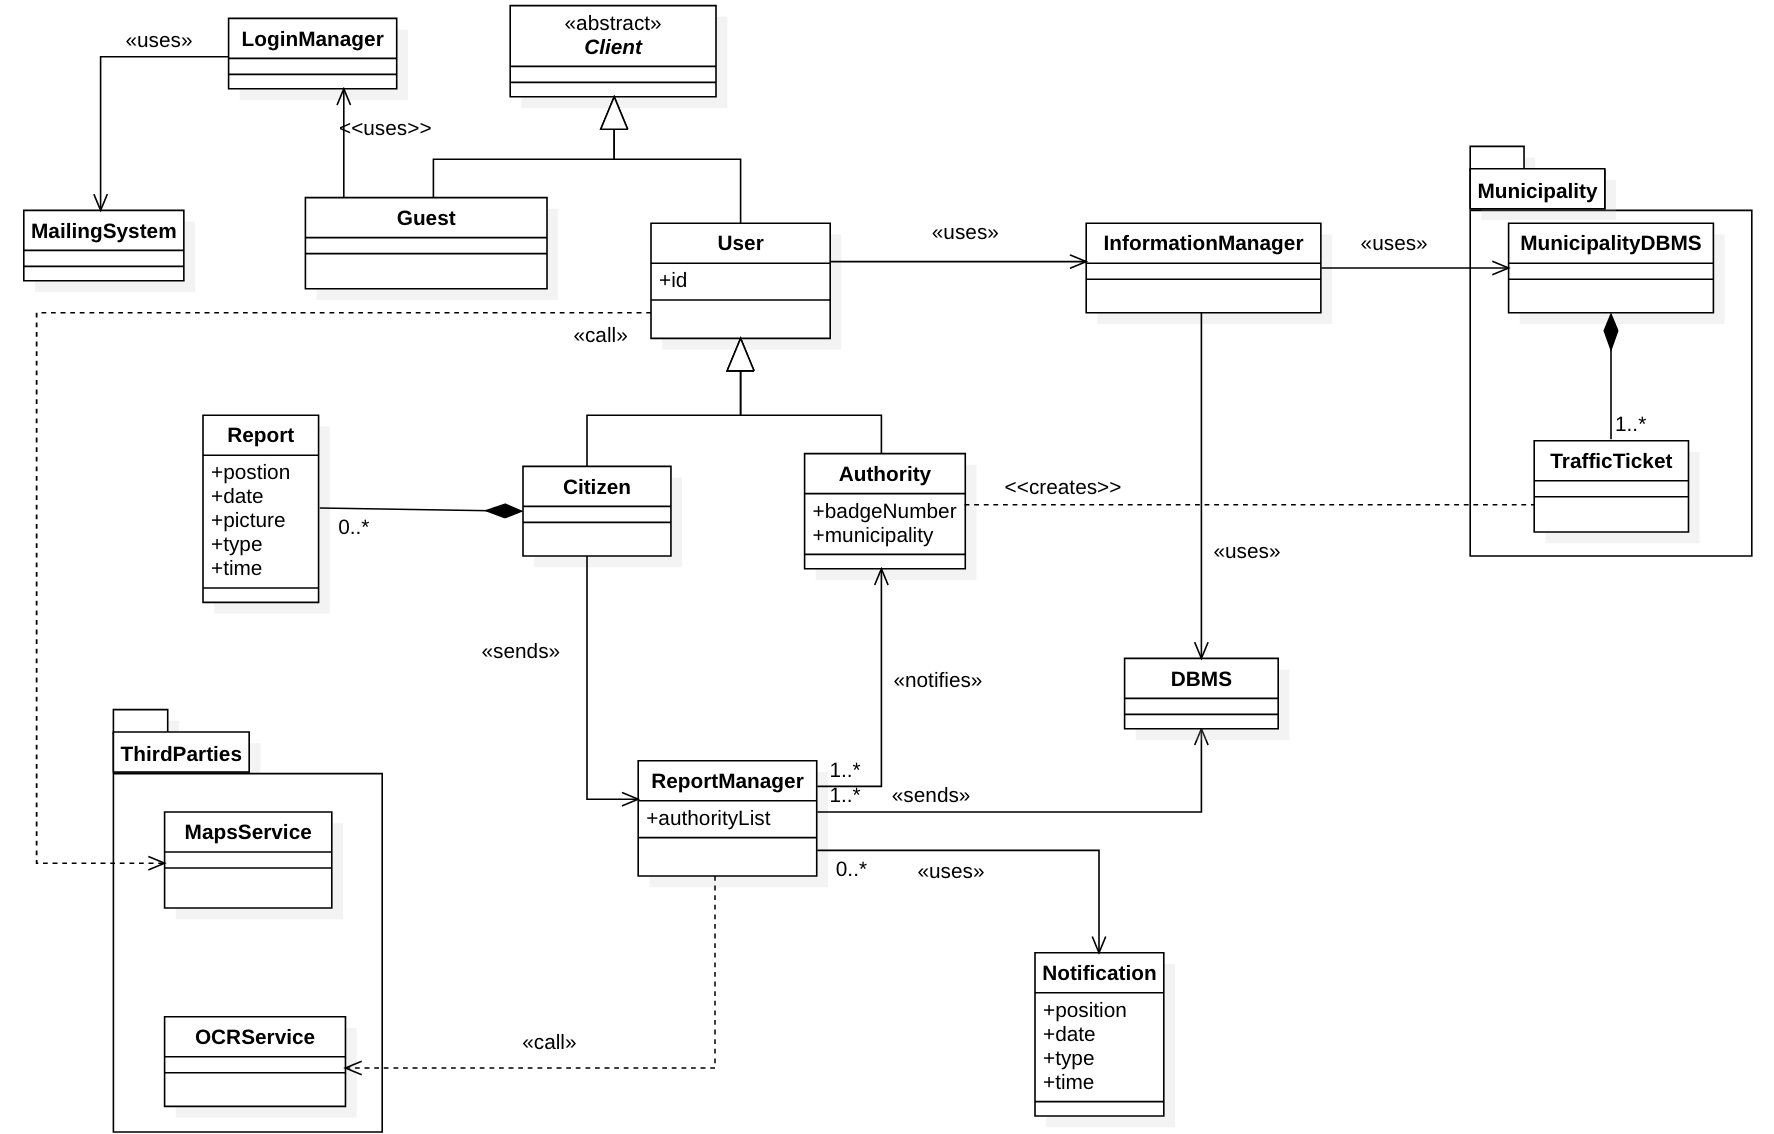
\includegraphics[width=\textwidth]{./img/SWE1.png}
\end{center}
\caption{SafeStreets' class diagram.}
\label{fig:UML}
\end{figure} 
\newpage

\section{Product Functions}
In this section the most important features of the application are extensively explained:
\begin{itemize}
	\item \textbf{Commit of a Report}: the System allows a Citizen to notify Authorities whenever a traffic violations occur. This function is achieved by compiling a Report with a picture of the violation, the date, time, position, and type of violation. Not all of these fields are always compulsory: for example, in the case the type of violation is \textit{accident}, only date, time and position are required. Once all the information is gathered and the report is sent to SafeStreets, the Report Manager goes in the \texttt{Verifying Information} status: it checks if all the obligatory fields have been compiled correctly, and then adds some useful metadata to the Report. Among the additional metadata, the systems takes note of whether or not the position has been provided by GPS, and also if the sender has added any license plate in the \texttt{Checking License Plate} status. If no license plate has been inserted, the Report Manager runs an OCR algorithm to retrive it from the picture provided (\texttt{Running OCR} status). \\
	After all the steps above, the Report is validated (\texttt{Validating Report} status) and a copy of it is notified to the Authorities, which we assume are going to handle it properly (g.e. dispatching a local police patrol). It is important to outline that the System is only designed to inform Authorities whenever a new report is confirmed, but by no means it provides a function which generates official traffic tickets or dispatches patrols in case of accidents. Also, it's relevant to notice that the Report Manager contains a list of all the Authorities, so it can notify all and only those Authorities who are on duty in the involved municipality. Finally, the Report is encrypted by means of a hash function (\texttt{Encrypting Report} status), thus no one can alter the information after its confirmation (see Section \ref{sec:security} for more details on security). \\
	Once the Report has been validated and encrypted the System is ready to store it: the Report is sent to the Storage Manager, where it's stored into a local buffer and there awaits to be exported into SafeStreets' database. Each day at a set time (g.e. between day/night shifts of the police) the System permanently stores all the Reports into the database. This mechanism takes advantages of the fact that one does not need fresh data to do general statistics, and in return it gives the possibility to schedule the Report storage when the System is not busy.

	\item \textbf{Build statistics}: the System analyzes the stored data to compute general statistics and returns useful information to the Users. This function is carried out by an Information Manager, which is in charge of retrieving, decrypting and elaborating the information available to the Storage Manager. In particular, the Information Manager periodically executes the following functions:
	\begin{enumerate}
		\item Compute a statistic which highlights the areas and vehicles with the highest frequency of violations.
		\item \label{func2} Identify potentially unsafe areas by analyzing Reports of accidents, and suggest possible interventions.
		\item \label{func3} Analyze traffic ticket trends to build statistics about the most recurrent offenders and the effectiveness of SafeStreets.
	\end{enumerate}
	Every User can request to see the latest result of the functions above as soon as they are available. Since both Citizen and Authorities have access to those results, it's really important to give them different levels of visibility, so that classified information doesn't end up in the hands of civilians (g.e vehicles with the highest frequency of violations and most recurrent offenders). It is also worth noting that some of the above functions are enhanced, or even enabled, only if the Municipality grants the Information Manager access to their database. In particular, the Function \ref{func2} can be enhanced by crossing Authorities' accident information with SafeStreets', whereas Function \ref{func3} is entirely enabled only if the System has access to traffic tickets data.

	\item \textbf{Safety Suggestionss}: the System is able to give Authorities suggestions to improve the safety of urban areas. This function is enabled by the Information Manager and the statistics previously built. In fact, observing for each area which kind of violations are more frequent and the trends of the accidents, the Information Manager runs an artificial intelligence to detect which solution is the most suitable for a given problem. Just like for the report storing process, these suggestions are updated when the System is less busy (g.e. at night) and a sufficient amount of fresh data is added to the database. Safety Suggestionss are downloaded by SafeStreets' application togeter with the latest statistics results, whenever they are requested. Despite this, it should be noted that only Authorities have access to such data, as they are assumed to be those who implement the suggestions in order to improve their service.
\end{itemize}

\section{User Characteristics}
SafeStreets can be used from both Citizens and Authorities. It is recommended for adult users, but there are no limitation of age. 
We take for granted that the Users have access to Internet and are able to install and use the mobile application.\\
The character are:
\begin{itemize}
	\item \textit{Guest}: anyone who downloads and opens the app but still has to sign
	up or log in. He/she cannot use any of the functions provided by SafeStreets.
	\item \textit{User}: a registered Guest who has to logged either as Citizen or as Authority. He/She is recognized by the System through an ID and can access any feature of the application granted for his/her role.
	\item \textit{Citizen}: someone who has logged-in with his credentials, which is recognized by the System through an ID. He/she can access to the personal data menu and add new reports.
	\item \textit{Authority}: someone who has logged-in with his credentials. He/she is notified every time a new Report regarding its municipality is stored by the System.
\end{itemize}

\section{Assumptions, Dependencies and Constraints}
\subsection{Assumptions}
\begin{itemize}
	\item {[D.1]} The registration mail is assumed to be correctly recieved by the User.
	\item {[D.2]} The System internal clock time used to provide notifications is correct.
	\item {[D.3]} When a little accident occurs there is no need to contact the Authorities, whereas when a dangerous accident happens Users are supposed to phone call the Authorities for a promptly intervention.
	\item {[D.4]} The Authorities are assumed to  take measures when they are notified about a new report.
	\item {[D.5]} After the first time, the System does not need to request the access to the Municipality's database as long as its permission is valid.
	\item {[D.6]} The statistics and suggestions are assumed to be consulted by Authorities periodically, in order to provide a better service.
	\item {[D.7]} Only specific components of the System is able to decrypt sensible data.
	\item {[D.8]} SafeStreets is not responsible of the traffic tickets generated by Authorities.
\end{itemize}
\subsection{Dependencies}
\begin{itemize}
	\item A DBMS is needed in order to store and retrieve Users’ Reports.
	\item Information on issued tickets (and possibly accidents) are provided by the Municipalities' database, which has limited access. 
	\item The OCR tool is provided by external thrid party services.
	\item An external Mailing Service is used to send confirmation mails.
	\item The Map service is provided by external an third party (which can be different by the one that provides the OCR tool).
	\item The system relies on an AI to analyze the data, build statistics and compute suggestions.
\end{itemize}
\subsection{Constraints} \label{constraints}
\begin{itemize}
	\item Smartphone equipped with an OS compatible with the application.
	\item Properly working Internet connection.
	\item The permission to acquire and store personal data must be given by the User. 
	\item Offer the possibility to the Users to delete their account.
	\item It is impossible to know if the tickets are generated thanks to SafeStreets, or if they are independent from the service.
	
\end{itemize}

\chapter{Specific Requirements}
\section{External Interface Requirement}
SafeStreets is a mobile based application. In the following sections a more detailed description of the application is given in terms of hardware, software and communication interfaces. There are also present some prototypes of User Interface through mockups.
\subsection{User Interface}
\begin{figure}[!ht]
	\begin{center}
	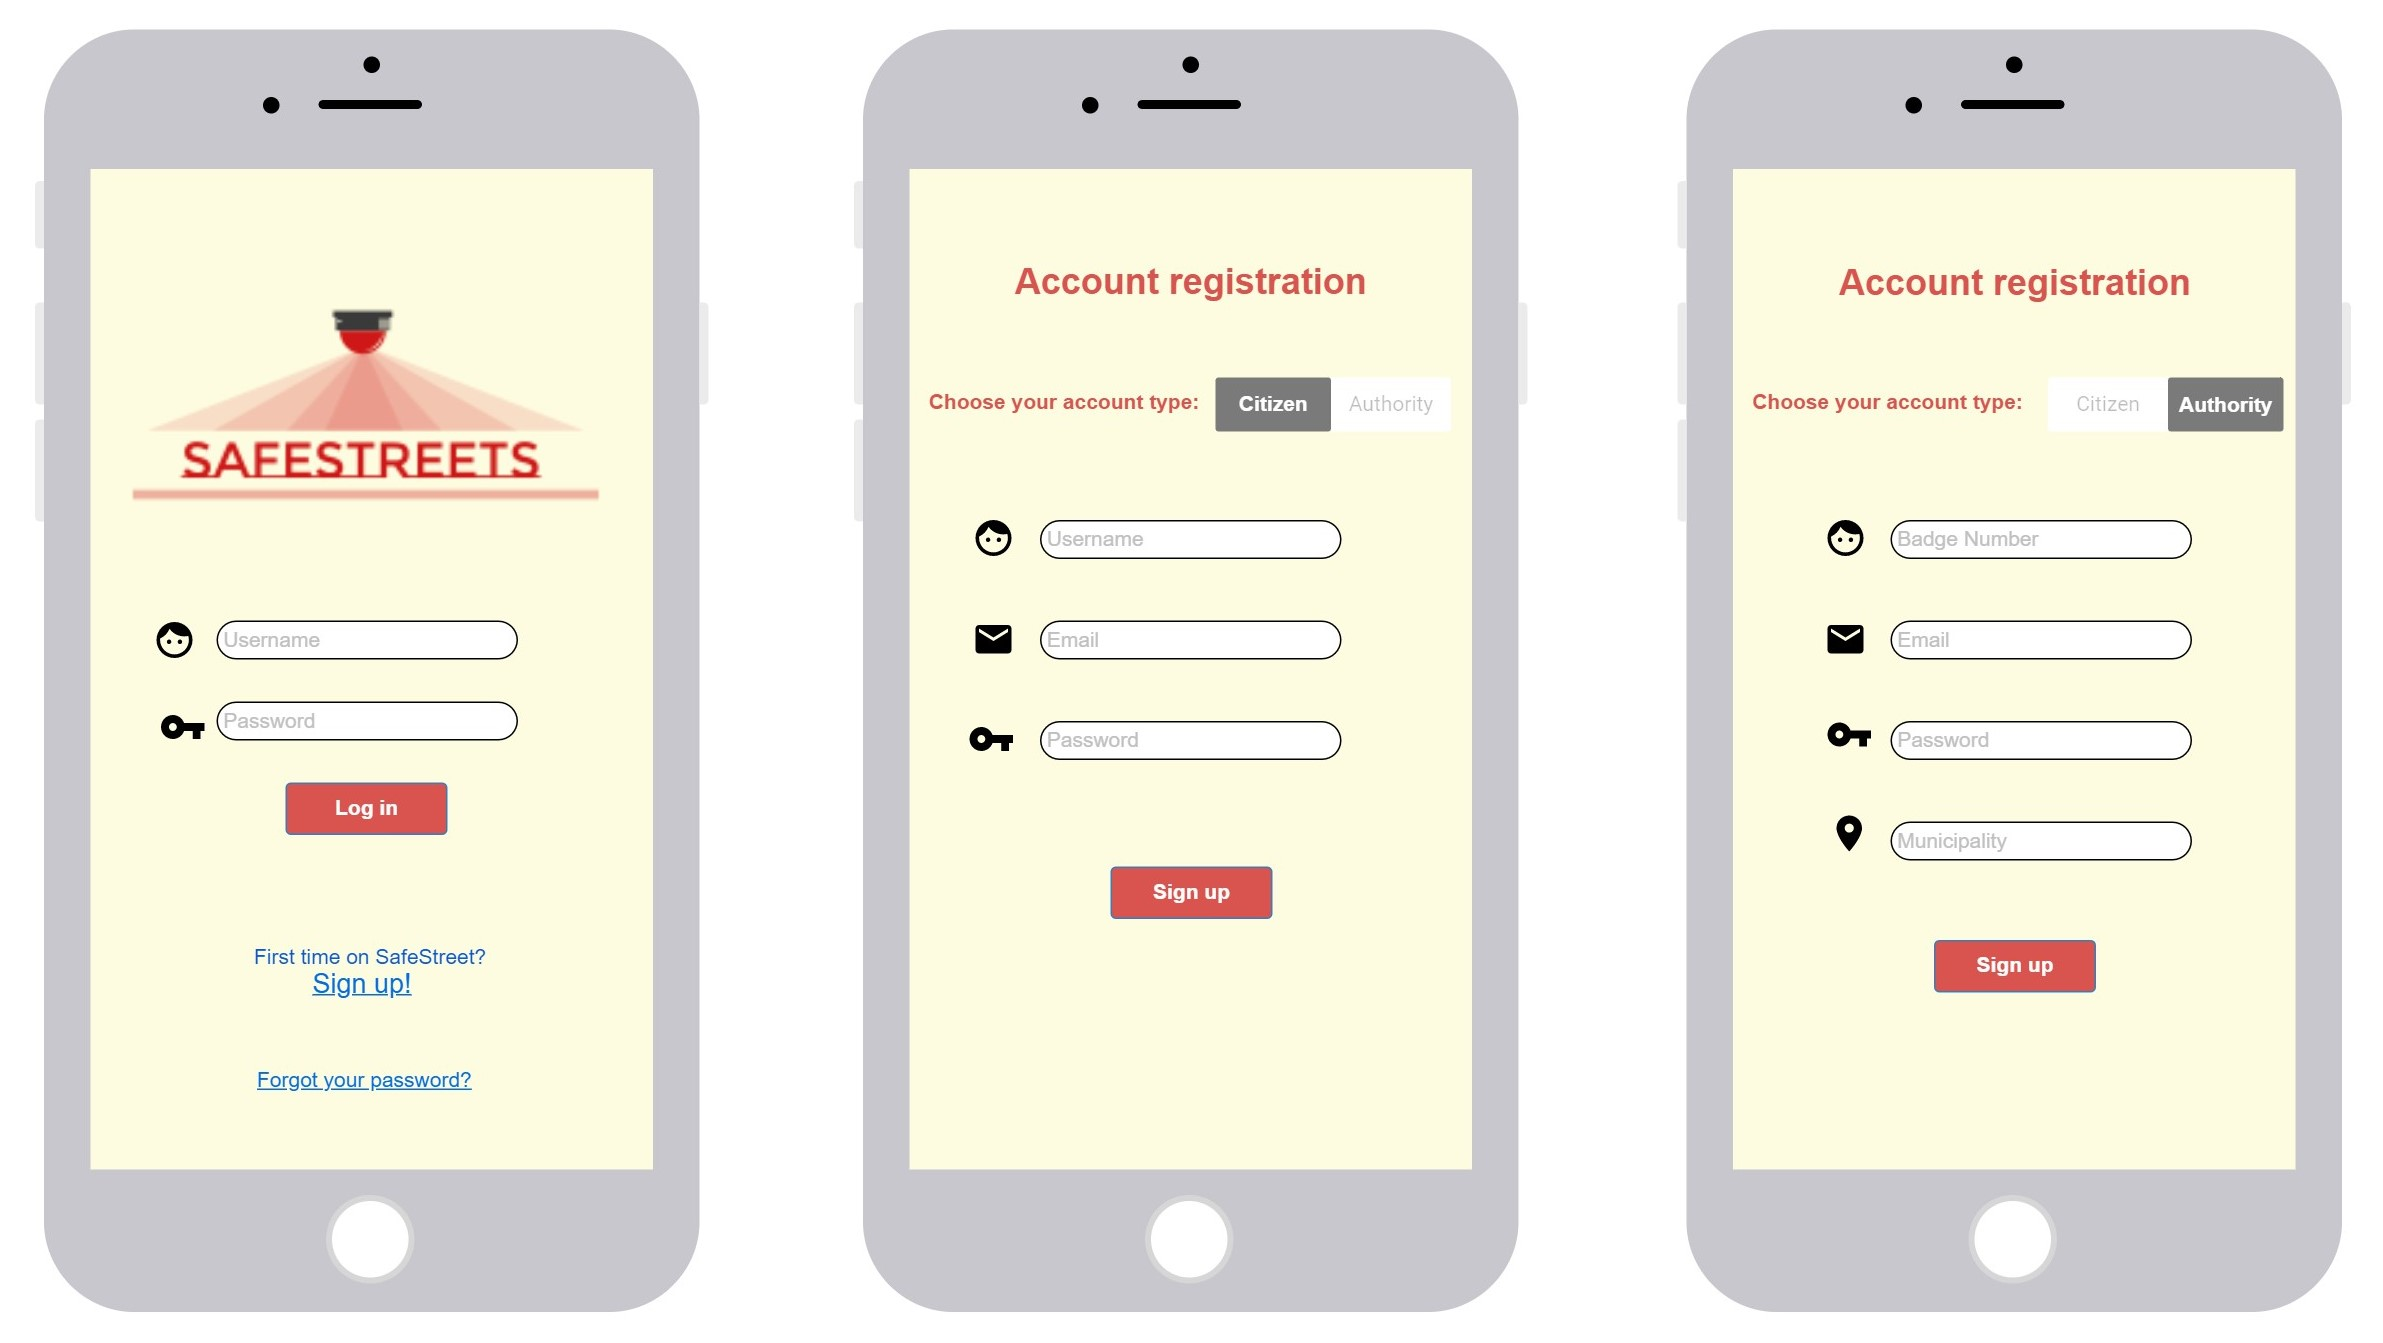
\includegraphics[width=\textwidth]{img/Mockup_logging.jpg}
	\end{center}
	\caption{Guest signup interface and login interface.}
\end{figure}
\begin{figure}[!htp]
	\begin{center}
	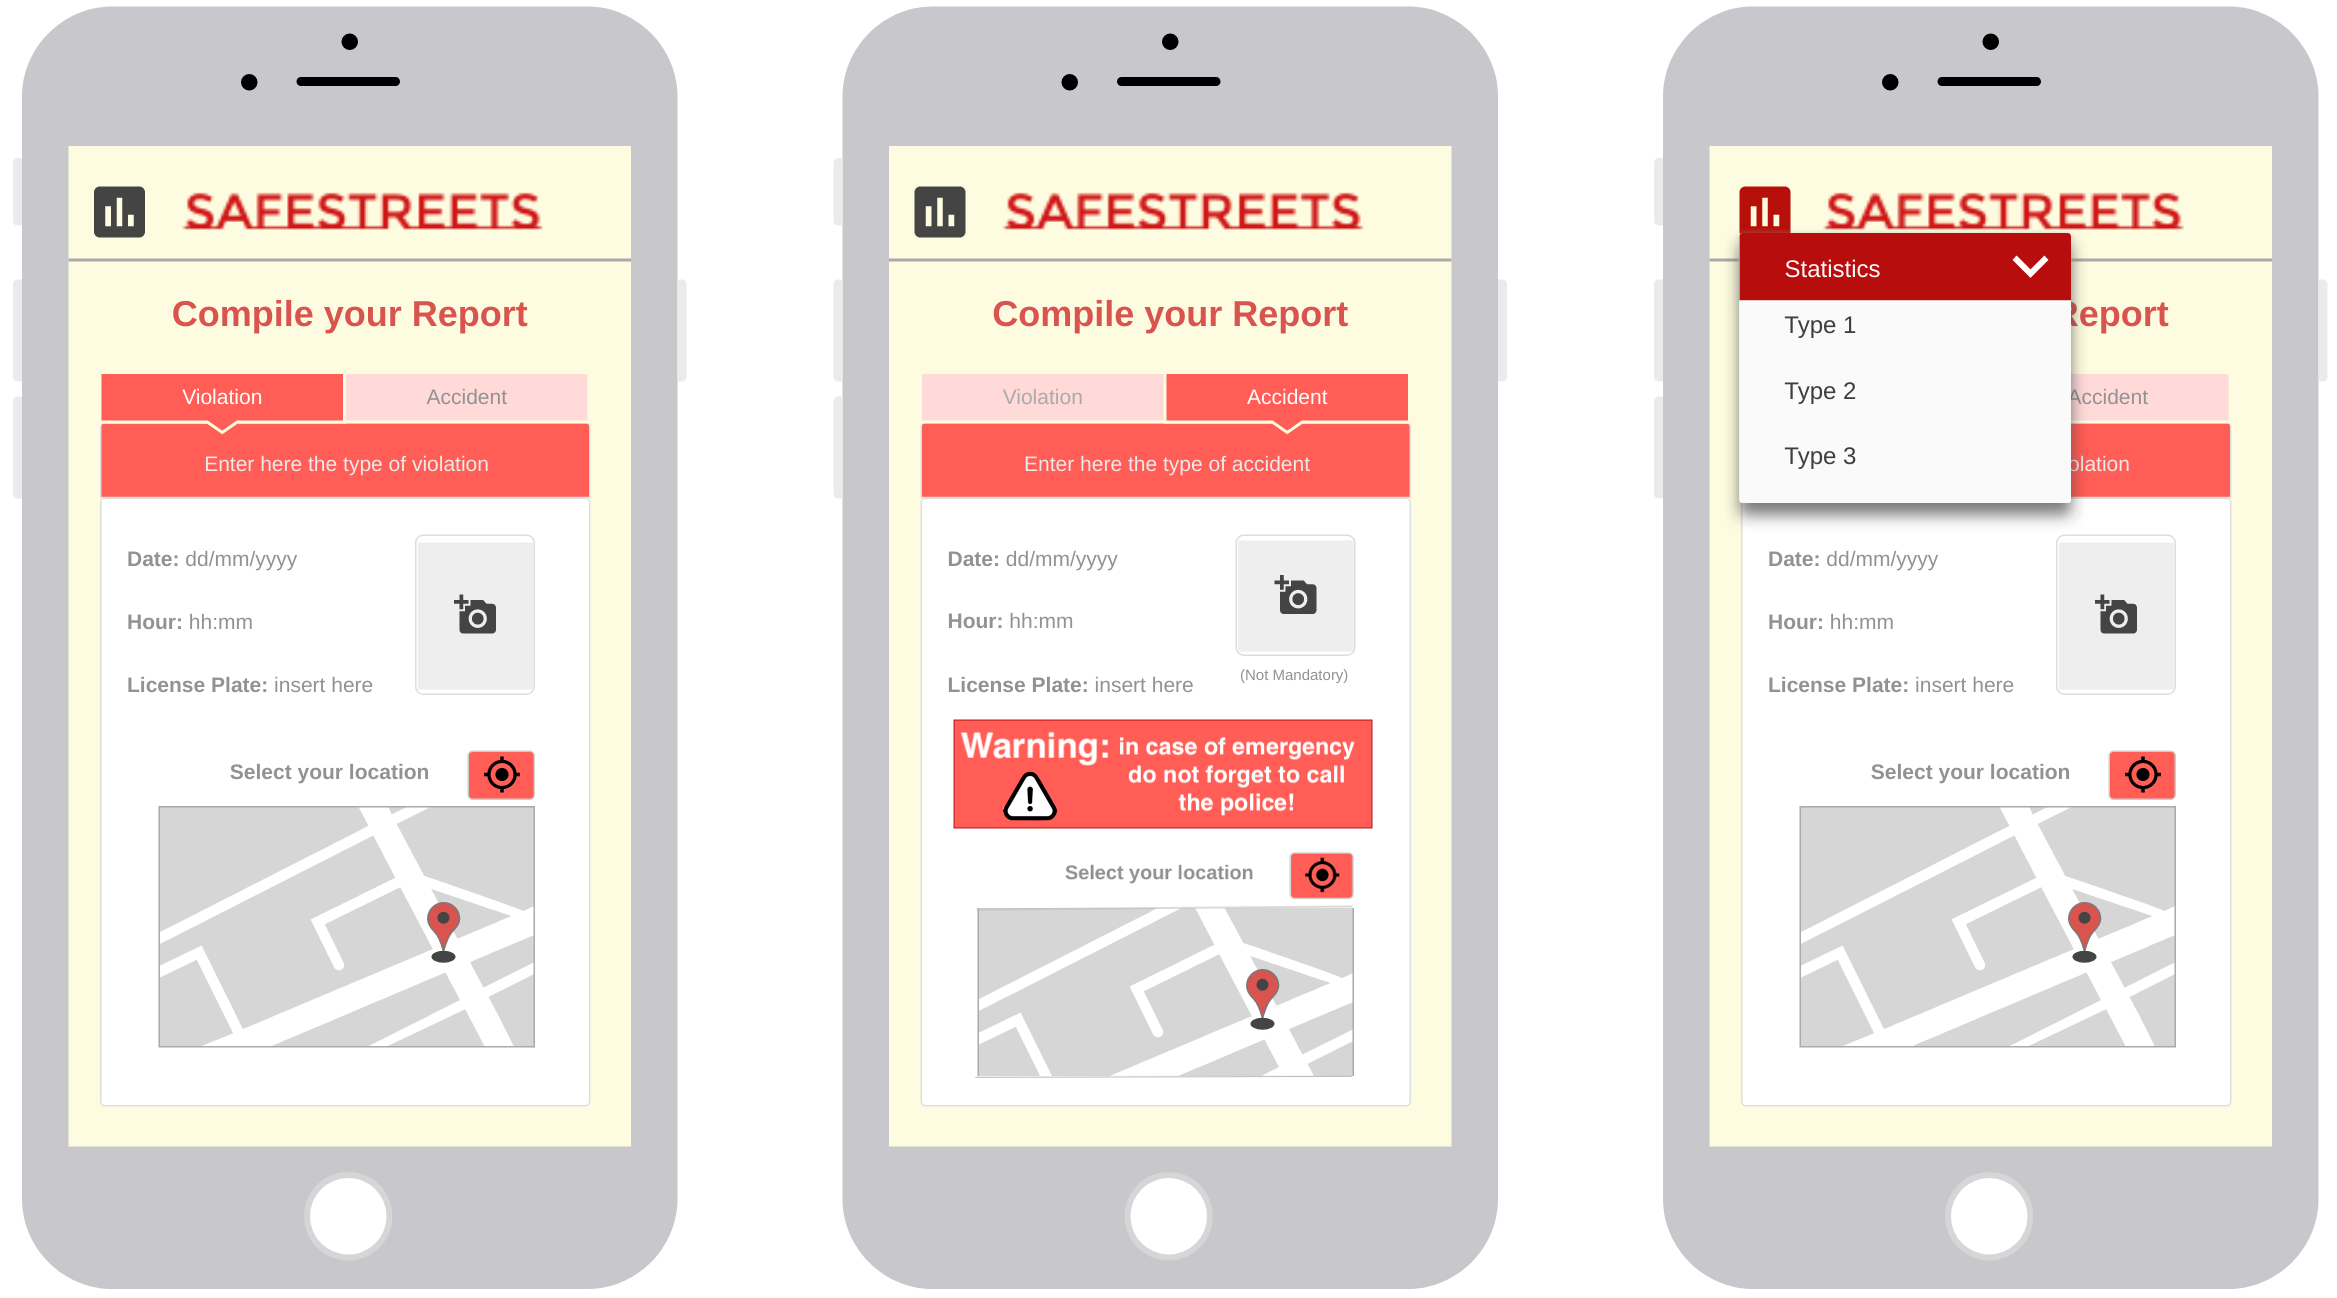
\includegraphics[width=\textwidth]{img/CitizensInterface.png}
	\end{center}
	\caption{Citizens interfaces to make new report (violation or accident), and to consult statistics menu.}
\end{figure}
\begin{figure}[!ht]
	\begin{center}
	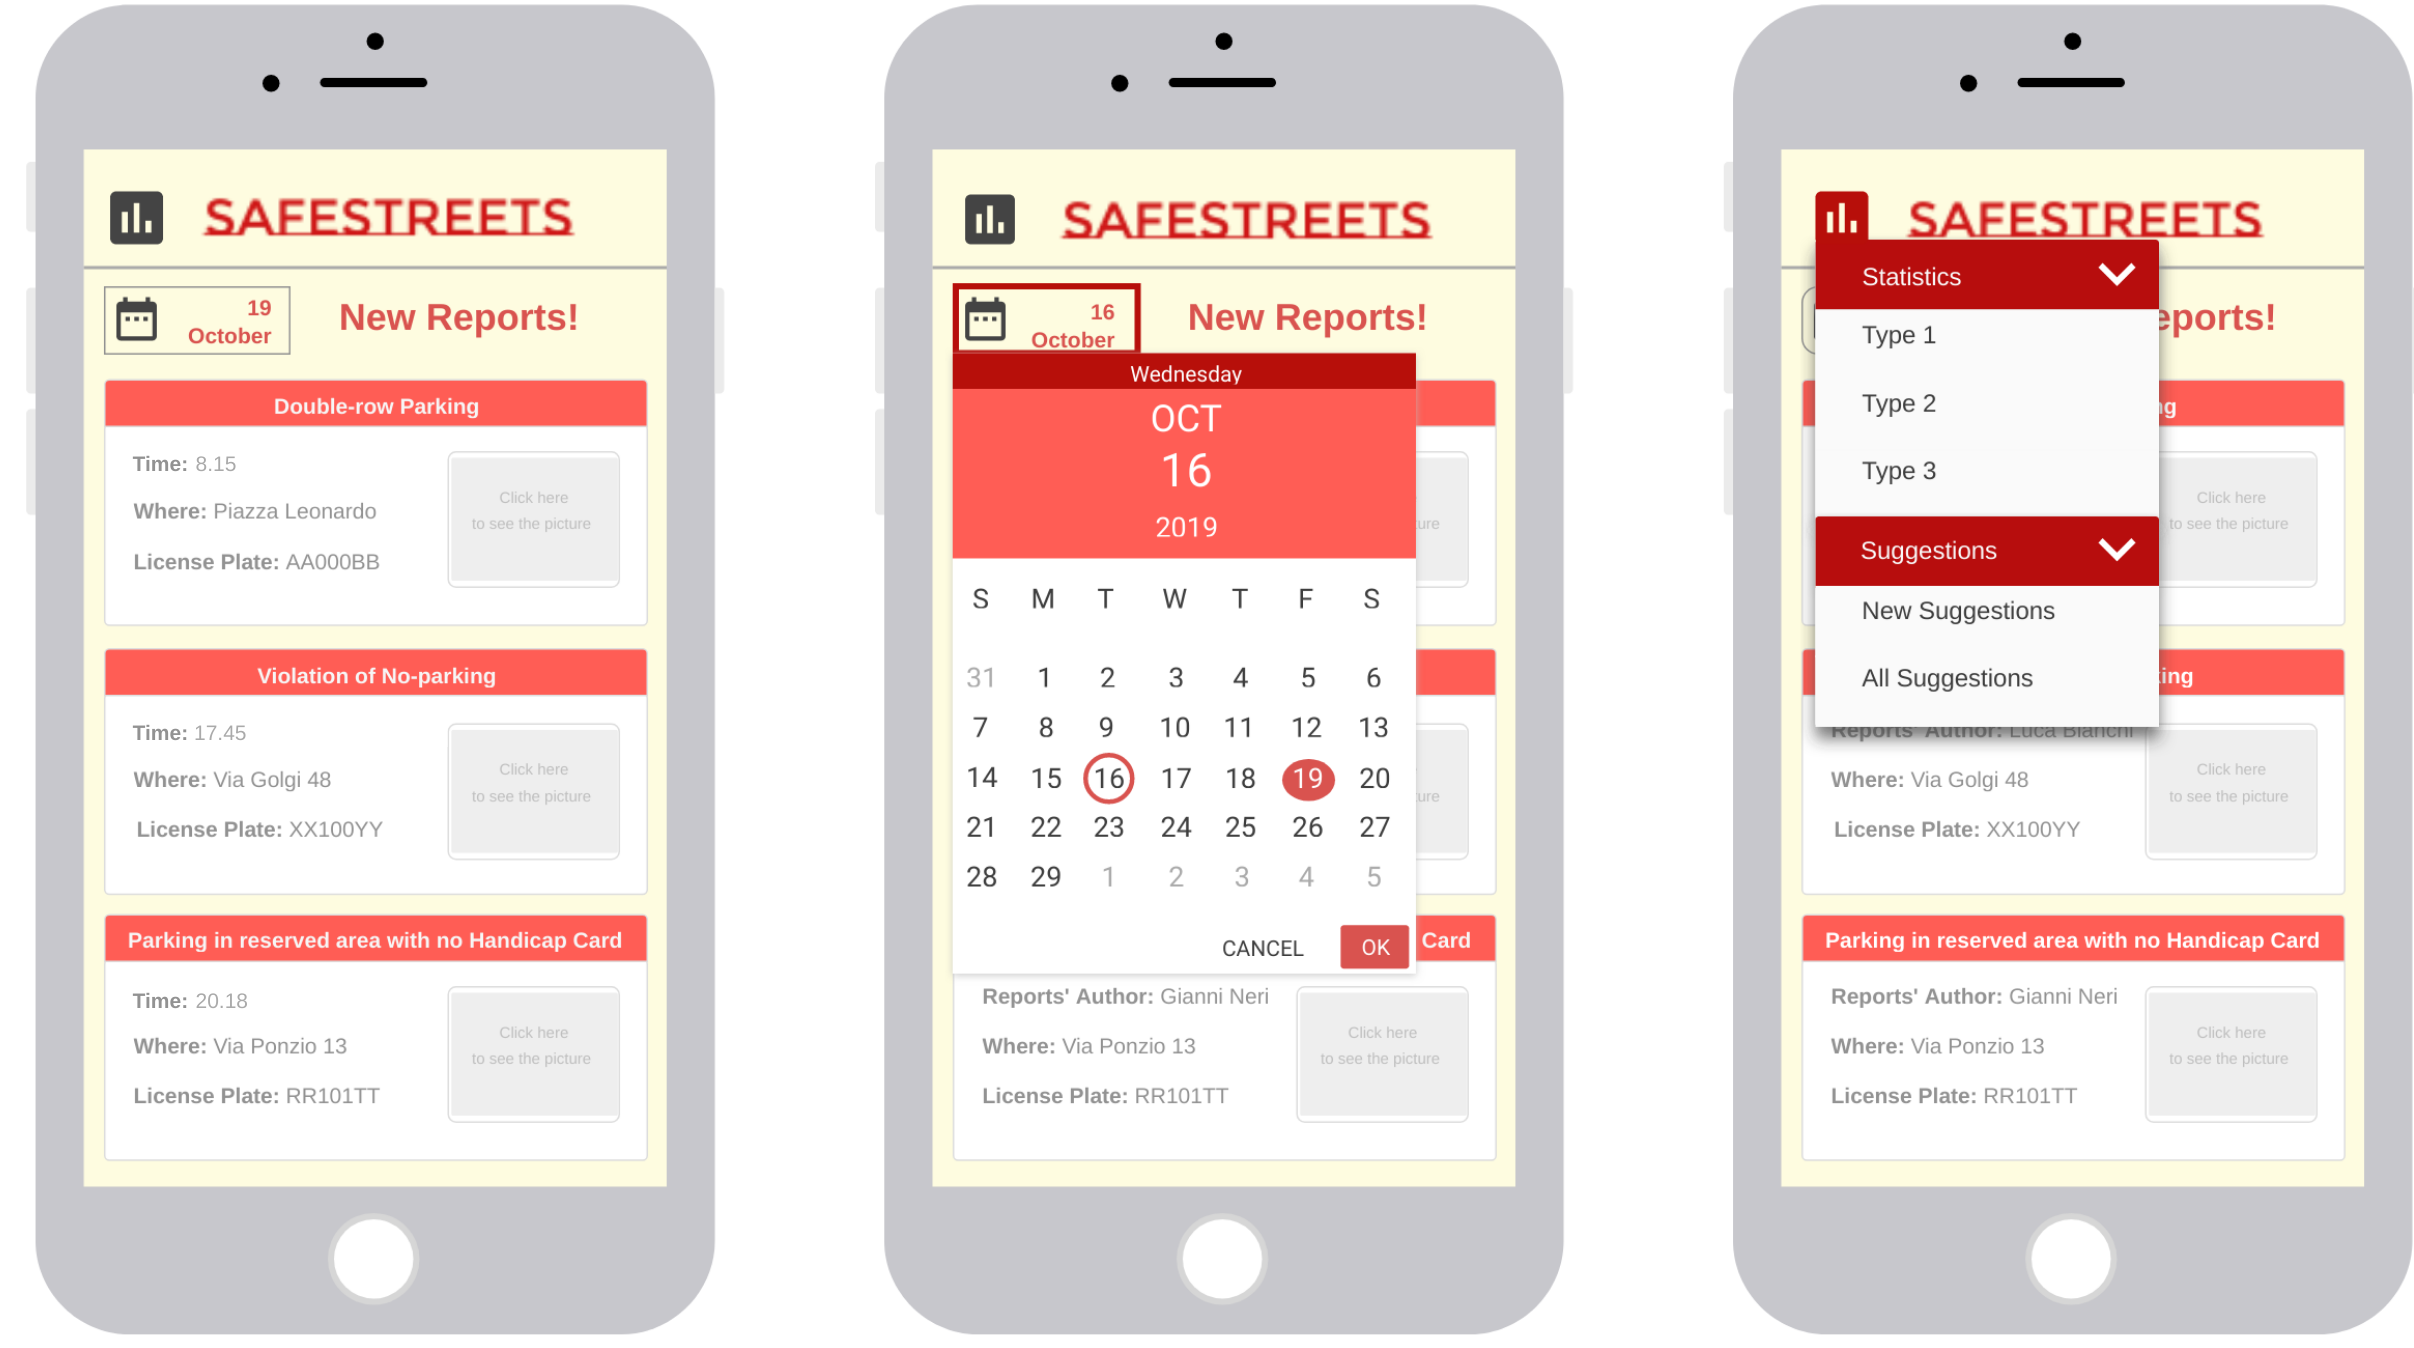
\includegraphics[width=\textwidth]{img/final.png}
	\end{center}
	\caption{Authorities interface to see new report, to consult statistics and suggestions menu.}
	\vfill
\end{figure}
\clearpage
\begin{figure}[!ht]
	\begin{center}
	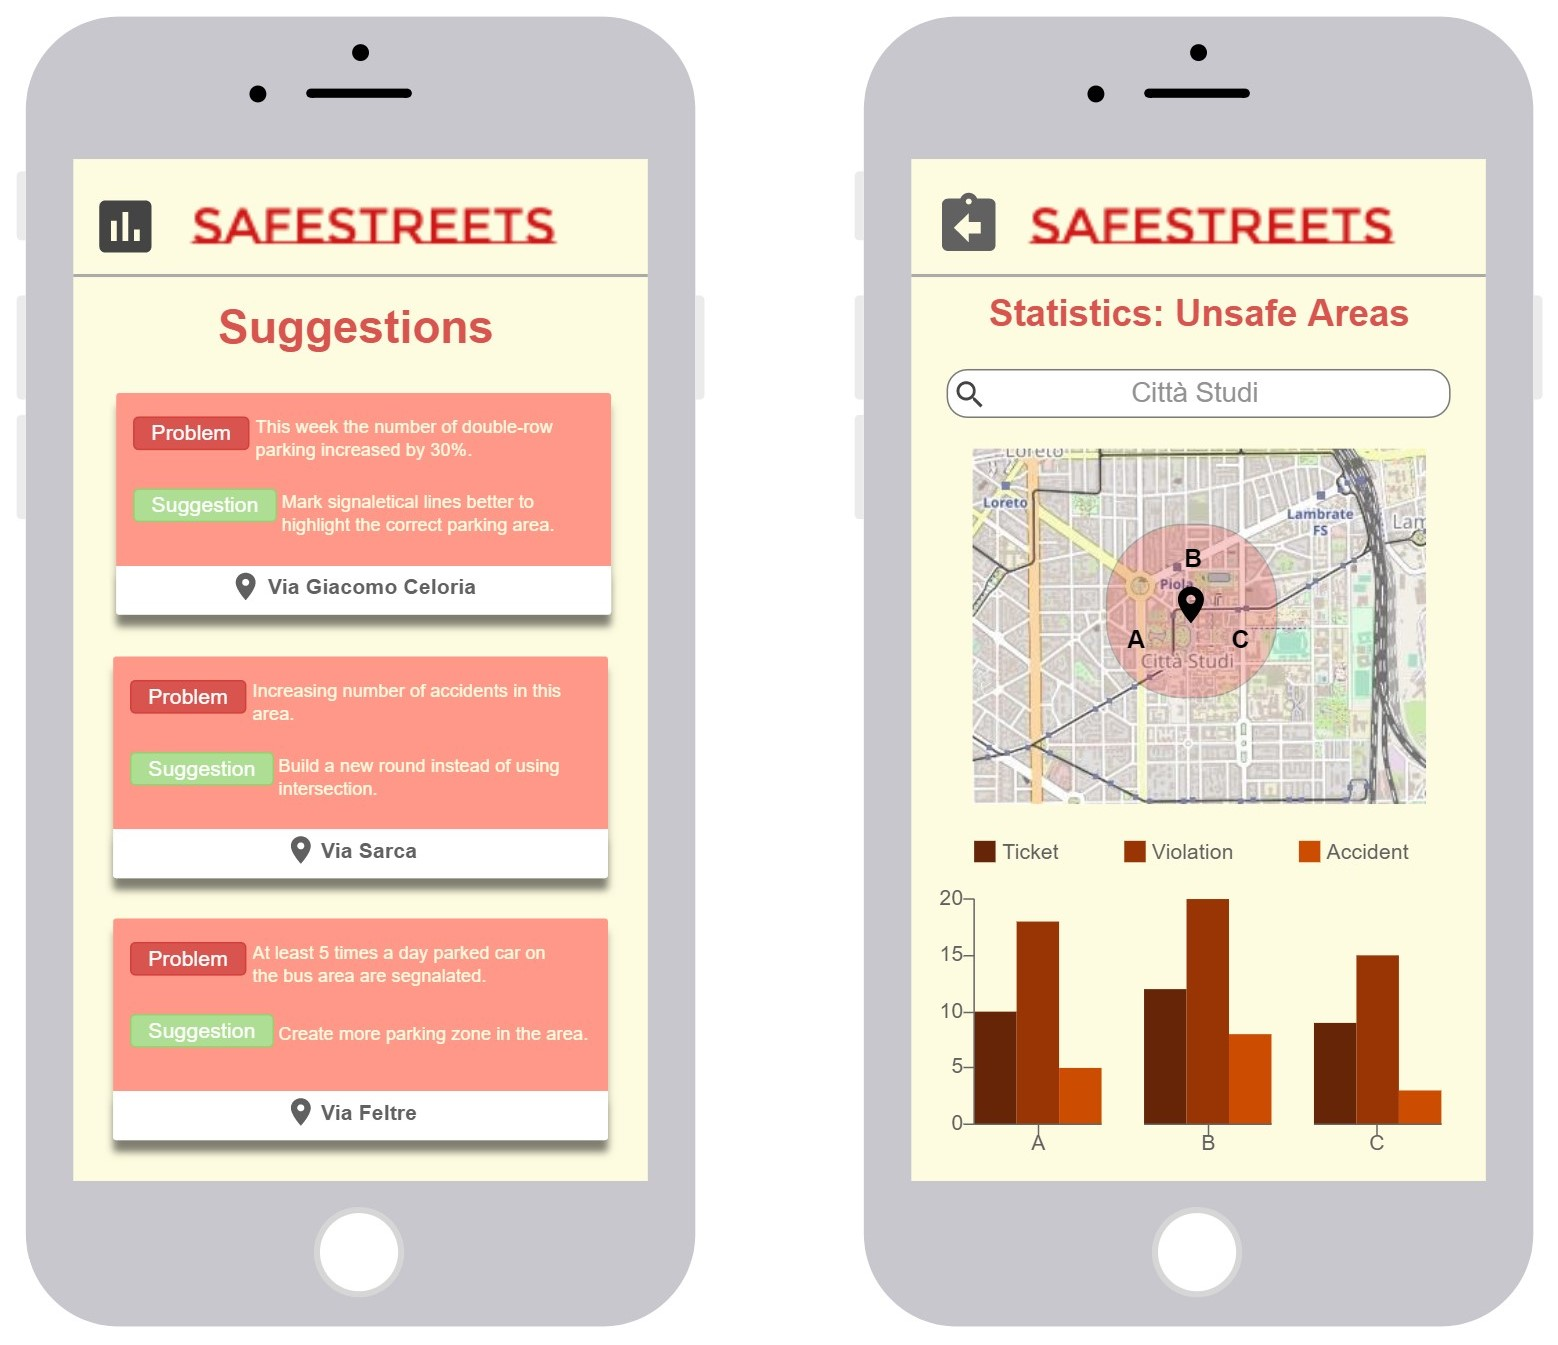
\includegraphics[width=0.7\textwidth]{img/StatisticsInterfaces.jpg}
	\end{center}
	\caption{Example of statistic and suggestion interfaces.}
\end{figure}

\subsection{Hardware Interface}
The application is avaiable for mobile devices that guarantee Internet access with a reasonably recent browser and have a camera with a fairly high definition.
\subsection{Software Interface}
\begin{itemize}
\item \textbf{Operating System}: iOS, Android.
\item Web browser.
\item Web Server application.
\item DBMS.
\item \textbf{Report System}: use third part services as OCR.
\item \textbf{Mailing Service}: APIs to send emails to the User.
\item \textbf{Mapping Service}: APIs to locate the position of the traffic violation.
\end{itemize}
\subsection{Communication Interface}
The application runs over HTTPS protocol for the communication over the Internet and with the DBMS.
\section{Functional Requirements}
In the following section are explained the functional requirements of the application.
\begin{itemize}
	\item {[R.1]} A visitor must be able to register. During the registration the System will ask to provide some credentials.
	\item {[R.2]} Check if the Guest credentials are valid:
		\begin{itemize}
			\item the username is not already taken by another registered User.
			\item the email is in the right format.
			\item the password has a minimum length.
			\item the badge is valid and matches the municipality, if the Guest is an Authority.
		\end{itemize}
	\item {[R.3]} If credentials are valid, the System sends a confirmation email..
	\item {[R.4]} Allow to log in using personal credentials.
	\item {[R.5]} Allow to change username, only if the new username is not already in use by another User, email, only if the
	new email is in a correct format and password, only if the new password is different from the precedent and respects the minimum length.
	\item {[R.6]} Send a confirmation email if username, email or password is changed (similarly to the registration process). 
	\item {[R.7]} Allow to change password if it has been forgotten, through the personal email.
	\item {[R.8]} The Citizen must be allowed to create reports, specifying:
		\begin{itemize}
			\item The type of report (violation/accident).
			\item The location of the violation/accident.
			\item The date of the violation/accident.
			\item The time of the violation/accident.
			\item A picture of the violation/accident (not mandatory).
		\end{itemize}
	\item {[R.9]} Check if the Report created by the Citizen is valid.
	\item {[R.10]} Notify the Authorities whenever a new Report involving their municipality is submitted. 
	\item {[R.11]} Provide two different level of visibility regarding the statistics. Only the Authorities can consult statistics with private data.
	\item {[R.12]} Safestreets' application must show the most recent version of the suggestions and statistics.
	\item {[R.13]} Provide a recognition system of badge number (this may involve communication with the Municipality).
	\item {[R.14]} Allow the Citizen to consult the history of its personal reports.
	\item {[R.15]} Allow Users to see the their position in a map.
	\item {[R.16]} All traffic violations must be notified to Authorities according to their municipality.
	\item {[R.17]} Provide the Authorities with a list of the most recent reports submitted.
	\item {[R.18]} Allow Authorities to also consult older Reports.
	\item {[R.19]} Interact with the Municipality's System to get the permission for using their data.
	\item {[R.20]} Use third party services to enable some functions (OCR and Mapping System).
	\item {[R.21]} Statistics and suggestions have to be periodically recomputed.
	\item {[R.22]} Provide protection of data using encryption.
	\item {[R.23]} Acknowledge whether or not multiple istances of Reports are referred to the same infraction, even if protracted over time.
	\item {[R.24]} Cross the data coming from external DBMS with the System's own data.
	\item {[R.25]} Cross data from different Reports in order to establish their truthfulness.
	\item {[R.26]} Unsafe areas are detected by means of an artificial intelligence.
	\item {[R.27]} Safety Suggestions are computed by means of an artificial intelligence.
	\item {[R.28]} After its validation, no one should be able to modify a submitted Report.
\end{itemize}

\newpage

\subsection{Use Cases}

\begin{figure}[ht!]
\begin{center}
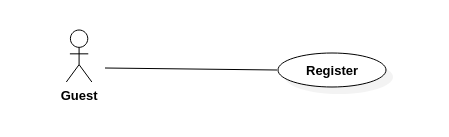
\includegraphics[width=\textwidth]{./img/UseCase1.png}
\end{center}
\caption{Guest use case.}
\label{fig:UseCase1}
\end{figure}
%%%%%%%%%%%%%%%%%%%%%%%%%%%%%%%%%%%%%%%%%%%%%%%%%%%%%%%
\begin{center}
	\textbf{Register Account}
\end{center}

\begin{tabularx}{\linewidth}{| l | X |}
	\hline
	\textbf{ID} & UC1\\
	
	\hline
	\textbf{Description} & The \textbf{\textit{Guest}} wants to create an account for the application.\\
	
	\hline
	\textbf{Achieved Goals} & {[G.1]}\\

	\hline
	\textbf{Actors} & \textbf{\textit{Guest}}, \textbf{\textit{Login Manager}} and \textbf{\textit{Mailing Service}}\\
	
	\hline
	\textbf{Preconditions} & The \textbf{\textit{Guest}} downloads and opens the application.\\
	
	\hline
	\textbf{Flow of Events} & \parbox{0.7\textwidth}{	
		\begin{enumerate}
			\item The \textbf{\textit{Guest}} taps the Sign Up button and and selects a role between Citizen or Authority.
			\item Based on the \textbf{\textit{Guests'}} decision, the \textbf{\textit{Login Manager}} provides the appropriate form to enter all the required data: username, email address and password. In the Authority's form the username corresponds to the badge number, and the municipality of belonging must be inserted as well. 
			\item The \textbf{\textit{Guest}} fills the form with all the required information and then confirms the entries. The same procedure will be used for future logins.
			\begin{itemize}
				\item If the \textbf{\textit{Guest}} is an Authority, he/she has to insert his/her badge number as username and provide the municipality of belonging.
			\end{itemize}	
			\item The \textbf{\textit{Login Manager}} checks if all the informa-
			tions are correct, in which case it generates a random activation
			URL and asks the \textbf{\textit{Mailing Service}} to forward the URL to the email address of the \textbf{\textit{Guest}}.
			\item The \textbf{\textit{Guest}} receives the mail and clicks on the URL. \item The \textbf{\textit{Login Manager}} accepts the registration and stores the data provided by the \textbf{\textit{User}} .
	\end{enumerate}}\\
	
	\hline
	\textbf{Postconditions} & The \textbf{\textit{Guest}} is now able to log in.\\
	
	\hline
	\textbf{Exceptions} & \parbox{0.7\textwidth}{ \begin{enumerate}
			\item The \textbf{\textit{Login Manager}} realizes that invalid cerdentials have been entered (g.e. the account already exists) and shows an error message. The flow restarts from point 2. 
		\end{enumerate}}\\

	\hline
	
\end{tabularx}

%%%%%%%%%%%%%%%%%%%%%%%%%%%%%%%%%%%%%%

\begin{center}
	\textbf{Log in}
\end{center}

\begin{tabularx}{\linewidth}{| l | X |}
	\hline
	\textbf{ID} & UC2\\
	
	\hline
	\textbf{Description} & The \textbf{\textit{Guest}} wants to log in to the application.\\

	\hline
	\textbf{Achieved Goals} & {[G.1]} and {[G.2]}\\
	
	\hline
	\textbf{Actors} & \textbf{\textit{Guest}} and \textbf{\textit{Login Manager}} \\
	
	\hline
	\textbf{Preconditions} & A \textbf{\textit{Guest}} wants to log in to the application and is already registered.\\
	
	\hline
	\textbf{Flow of Events} & \parbox{0.7\textwidth}{
		\begin{enumerate}
			\item The \textbf{\textit{Guest}} opens the application and inserts his/her credentials (username and password).
			\begin{itemize}
				\item If the \textbf{\textit{Guest}} is an Authority, he/she has to insert his/her badge number as username.
			\end{itemize}
			\item The \textbf{\textit{Guest}} taps the Log In button.			
			\item The \textbf{\textit{Login Manager}} checks if all the credentials provided are correct.
	\end{enumerate}}\\
	
	\hline
	\textbf{Postconditions} & The \textbf{\textit{User}} is logged in either as Citizen or Authority.\\
	
	\hline
	\textbf{Exceptions} & \parbox{0.7\textwidth}{ 
		\begin{enumerate}
			\item The \textbf{\textit{Login Manager}} recognizes invalid credentials than shows an error message. The flow restarts from point 1. 
		\end{enumerate}}\\
	
	\hline
\end{tabularx}
%%%%%%%%%%%%%%%%%%%%%%%%%%%%%%%%%%%%%%%%%%%%%%%%%%
\begin{figure}[ht!]
\begin{center}
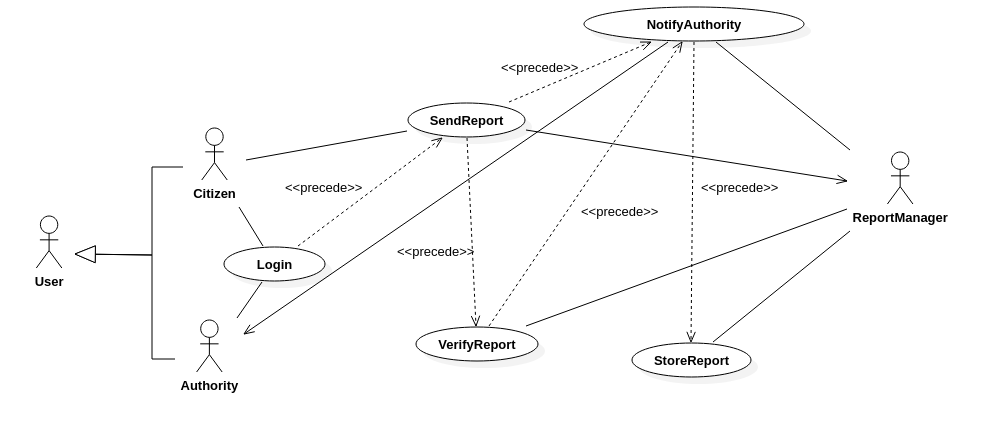
\includegraphics[width=\textwidth]{./img/UseCase2.png}
\end{center}
\caption{User and Report Manager use case.}
\label{fig:UseCase2}
\end{figure}

\begin{center}
	\textbf{Send report}
\end{center}

\begin{tabularx}{\linewidth}{| l | X |}
	\hline
	\textbf{ID} & UC3\\
	
	\hline
	\textbf{Description} & A \textbf{\textit{Citizen}} reports a traffic violation.\\
	
	\hline
	\textbf{Achieved Goals} & {[G.3]} and {[G.4]}\\

	\hline
	\textbf{Actors} & \textbf{\textit{Citizen}} and \textbf{\textit{Report Manager}}\\
	
	\hline
	\textbf{Preconditions} & The \textbf{\textit{Citizen}} witnesses a traffic violation and wants to report it.\\
	
	\hline
	\textbf{Flow of Events} & \parbox{0.7\textwidth}{\begin{enumerate}
			\item The \textbf{\textit{Citizen}} logs in to the application.
			\item The \textbf{\textit{Citizen}} taps on \textit{Report} button.
			\item The \textbf{\textit{Citizen}} compiles a Report.
			\begin{itemize}
				\item He/She takes a picture of the violation, if possible.
				\item He/She also enters the date, time, location and the type of the violation.			
			\end{itemize}
			\item The \textbf{\textit{Citizen}} taps the \textit{Send} button.
			\item The \textbf{\textit{Report Manager}} checks if the report has been correctly compiled.		
	\end{enumerate}}\\
	
	\hline
	\textbf{Postconditions} & The report is sent and the \textbf{\textit{Citizen}} recives a message that confirms the sending was successful.\\
	
	\hline
	\textbf{Exceptions} & \parbox{0.7\textwidth}{ \begin{enumerate}
			\item The \textbf{\textit{Report Manager}} rejects the report and shows an error message saying what fields are wrongly compiled. The flow restarts from point 2. 
		\end{enumerate}}\\
	
	\hline
	
\end{tabularx}
%%%%%%%%%%%%%%%%%%%%%%%%%%%%%%%%%%%%%%%%%%%%%%%%%
\begin{center}
	\textbf{Store and Notify report}
\end{center}

\begin{tabularx}{\linewidth}{| l | X |}
	\hline
	\textbf{ID} & UC4\\
	
	\hline
	\textbf{Description} & The \textbf{\textit{Report Manager}} recieves a report from a Citizen and notifies the Authorities about it. Then the report is stored in a database.\\
	
	\hline
	\textbf{Achieved Goals} & {[G.4]} and {[G.5]}\\

	\hline
	\textbf{Actors} & \textbf{\textit{Report Manager}} and \textbf{\textit{Storage Manager}}\\
	
	\hline
	\textbf{Preconditions} & The \textbf{\textit{Report Manager}} recives a valid report (see UC3).\\
	
	\hline
	\textbf{Flow of Events} & \parbox{0.7\textwidth}{\begin{enumerate}
			\item The \textbf{\textit{Report Manager}} computes metadata (g.e. whether or not license plate has been entered, if position has been provided by GPS, etc.) and attaches them to the Report.
			\item The \textbf{\textit{Report Manager}} runs an API call to retrieve any information about the license plate by means of an external OCR.
			\item The \textbf{\textit{Report Manager}} notifies the Authorities of the municipality where the violation occurred about the report.
			\item The \textbf{\textit{Report Manager}} encrypts the report.	
			\item The \textbf{\textit{Report Manager}} sends the report to the \textbf{\textit{Storage Manager}}.
			\item The \textbf{\textit{Storage Manager}} stores the reports in the DBMS according to its schedule.
			
	\end{enumerate}}\\
	
	\hline
	\textbf{Postconditions} & The \textbf{\textit{Authorities}} are notified about the Report, which is now stored into the DBMS and ready to be analyzed for building statistics.\\
	
	\hline
	\textbf{Exceptions} & \parbox{0.7\textwidth}{ \begin{enumerate}
			\item If the type of the Report recived by the \textbf{\textit{Report Manager}} is \textit{Accident} the report is not notified to the authorities, but it is only stored in the database. 
		\end{enumerate}}\\
	
	\hline
	
\end{tabularx}

%%%%%%%%%%%%%%%%%%%
\begin{figure}[ht!]
	\begin{center}
	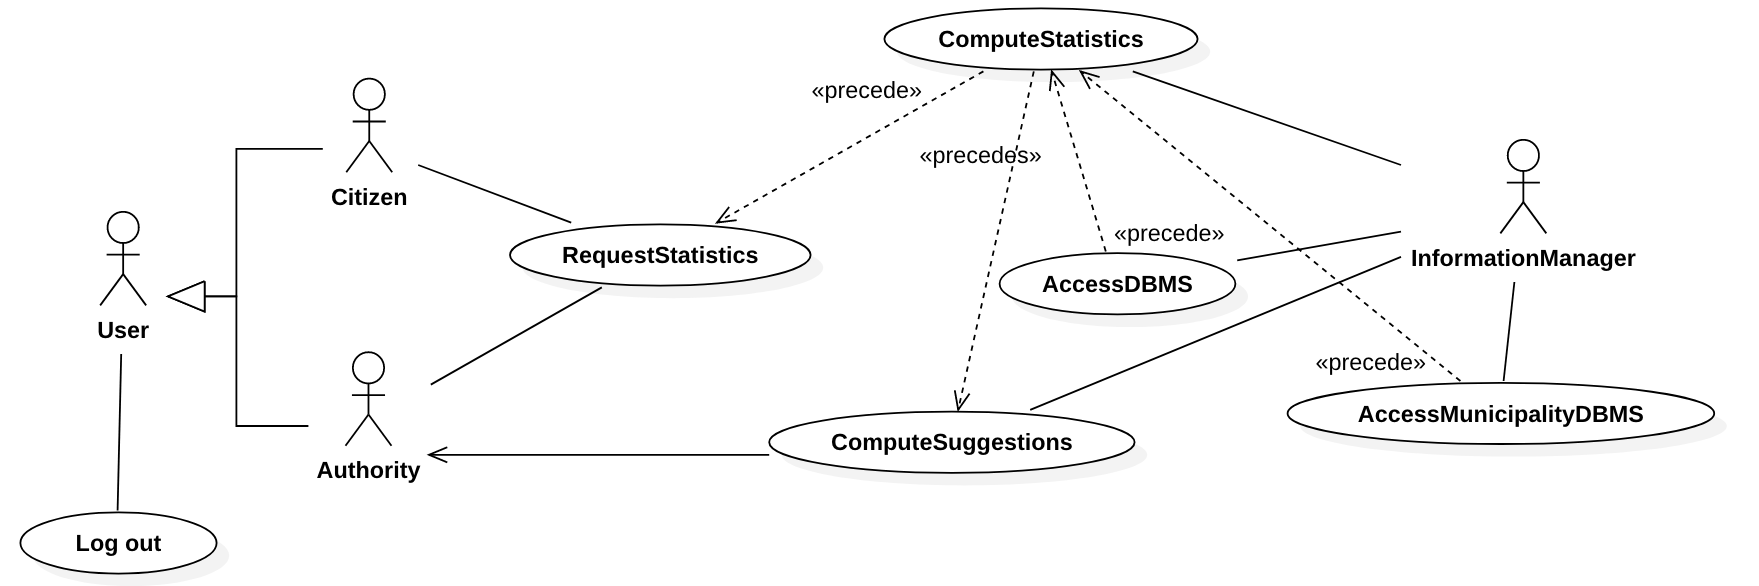
\includegraphics[width=\textwidth]{./img/UseCase3.png}
	\end{center}
	\caption{Information Manager use case.}
	\label{fig:UseCase3}
	\end{figure}
	\newpage
%%%%%%%%%%%%%%%%%%%%

\begin{center}
	\textbf{Compute Statistics}
\end{center}
\begin{tabularx}{\linewidth}{| l | X |}
	\hline
	\textbf{ID} & UC5\\
	
	\hline
	\textbf{Description} & A \textbf{\textit{User}} wants to see some statistics (e.g the safety of a certain area) and ask the \textbf{\textit{Information Manager}} about them.\\
	
	\hline
	\textbf{Achieved Goals} & {[G.6]}, {[G.7]}, {[G.8]}, and {[G.9]}\\

	\hline
	\textbf{Actors} & \textbf{\textit{User}} and \textbf{\textit{Information Manager}}\\
	
	\hline
	\textbf{Preconditions} & The \textbf{\textit{Information Manager}} has already computed the statistics that the user intends to consult. At set times, the \textbf{\textit{Information Manager}} updates all the statistics due to possible new stored reports. \\
	
	\hline
	\textbf{Flow of Events} & \parbox{0.7\textwidth}{\begin{enumerate}
			\item The \textbf{\textit{User}} logs in to the application and taps on the \textit{Statistics} button.
			\item The \textbf{\textit{System}} displays a menu with all the possible statistic options to compute.
			\item The \textbf{\textit{User}} chooses the statistics in which he/she is interested in.
			
			\item The \textbf{\textit{Information Manager}} loads the statistics that the user selected and the application shows them. 
			\begin{itemize}
				\item The application may use external services to show some statistics on a map.
				\item If the \textbf{\textit{User}} who requested to see the statistics is a Citizen, he/she should not be able to see statistics on sensible data.
				\item If the \textbf{\textit{User}} who requested to see the statistics is an Authority, the \textbf{\textit{Information Manager}} will also show him/her the latest safety suggestions (if available).
			\end{itemize}
			
	\end{enumerate}}\\
	
	\hline
	\textbf{Postconditions} & The \textbf{\textit{User}} sees the results of the statistics request.\\
	
	\hline
	\textbf{Exceptions} & \parbox{0.7\textwidth}{ \begin{enumerate}
			\item If the Municipality doesn't allow the Storage Manager to access their information, the \textbf{\textit{Information Manager}} use those data to build statistics. In this case, a message saying \textit{Statistic Unavailable} is shown to the \textbf{\textit{User}} who requests to see statistics about iussued traffic tickets. The flow restart from point 3.  
		\end{enumerate}}\\
	
	\hline
	
\end{tabularx}
%%%%%%%%%%%%%%%%%%%%%%%%
\newpage
\subsection{Sequence Diagrams}
\begin{figure}[ht!]
	\begin{center}
	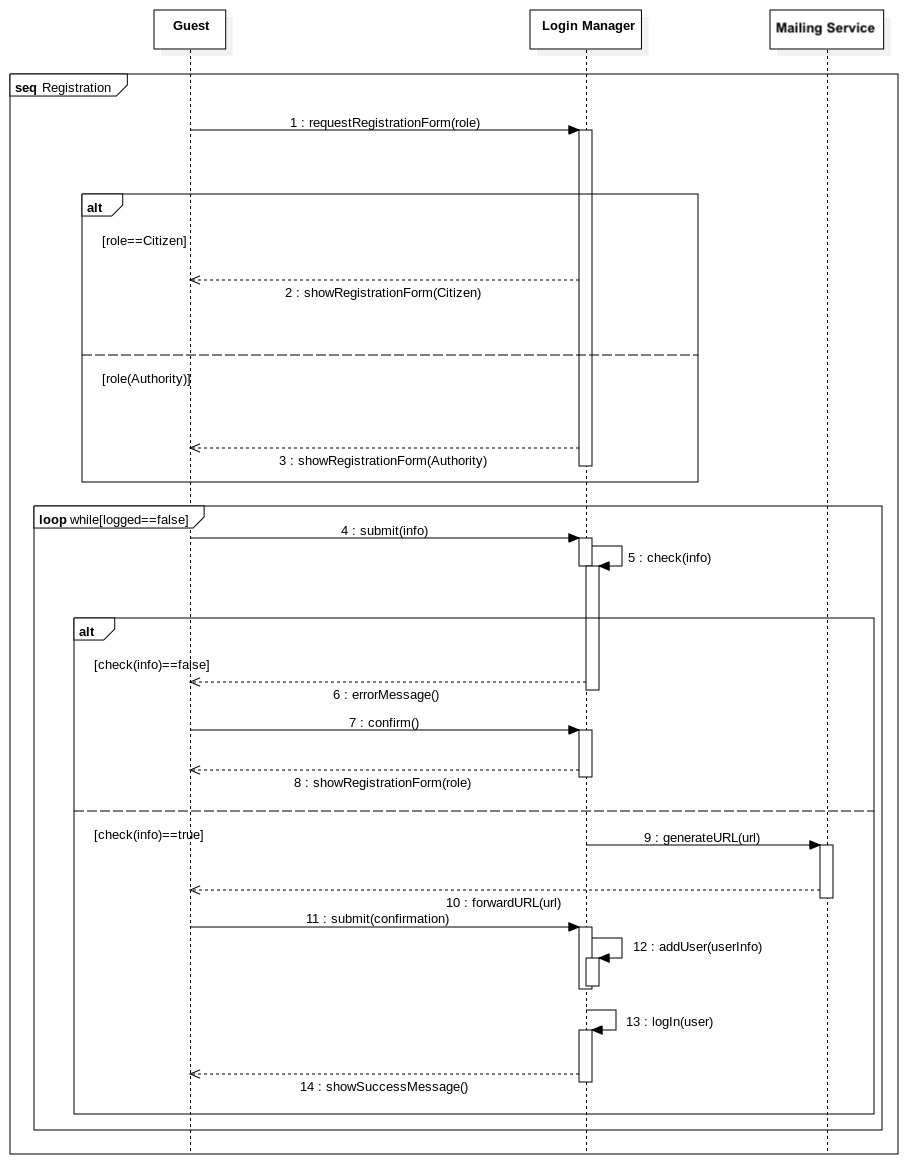
\includegraphics[width=\textwidth]{./img/RegistrationSD.png}
	\end{center}
	\caption{Sign up Sequence Diagram.}
	\label{fig:SequenceDiagram1}
	\end{figure}
\newpage
\begin{figure}[ht!]
\begin{center}
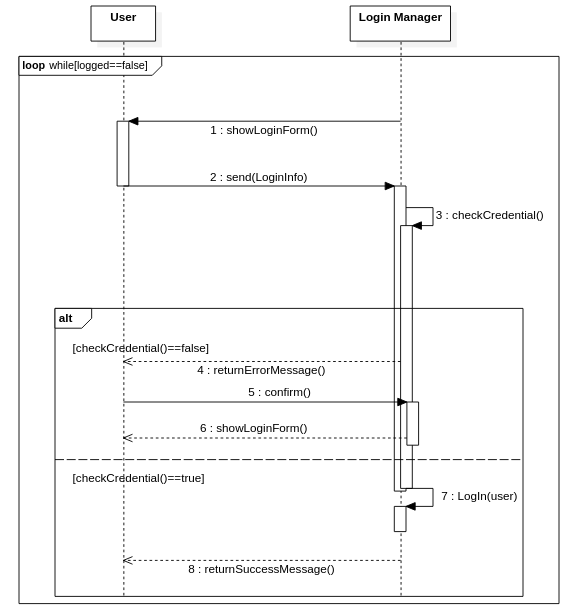
\includegraphics[width=\textwidth]{./img/LoginSD.png}
\end{center}
\caption{Login Sequence Diagram.}
\label{fig:SequenceDiagram2}
\end{figure}
\newpage
\begin{figure}[ht!]
\begin{center}
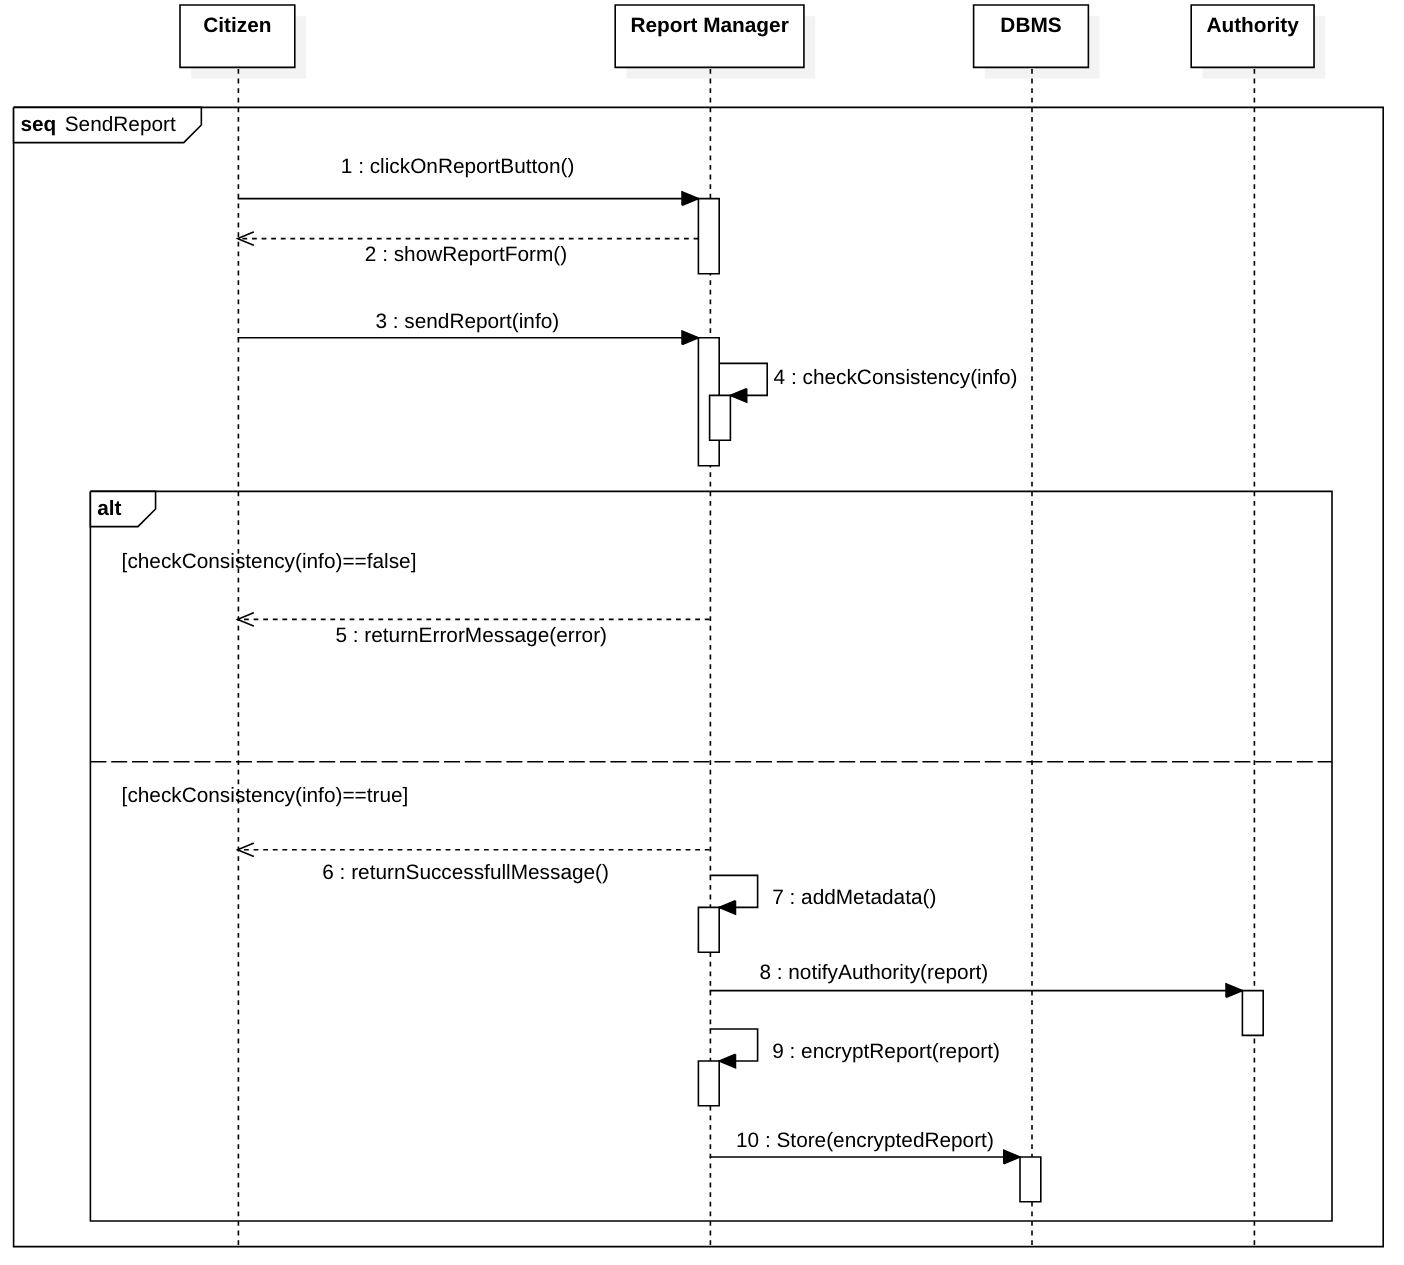
\includegraphics[width=\textwidth]{./img/SendReportSD.png}
\end{center}
\caption{Send Report, notify and Store report Sequence Diagram.}
\label{fig:SequenceDiagram3}
\end{figure}
\newpage
\begin{figure}[ht!]
\begin{center}
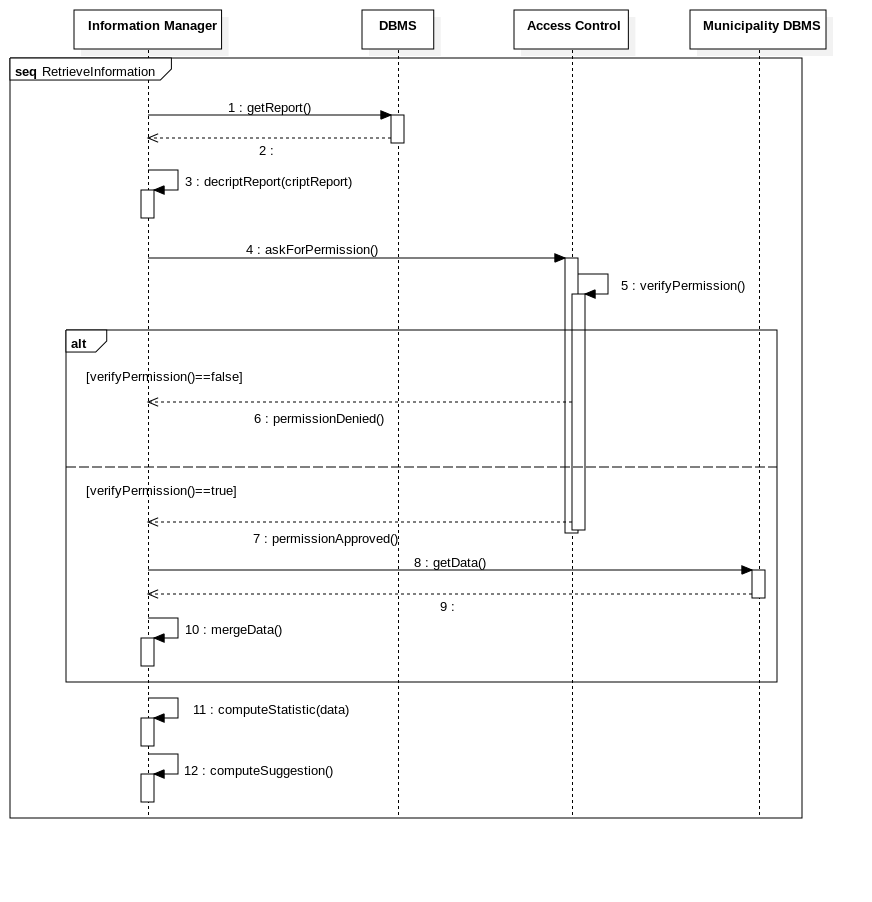
\includegraphics[width=\textwidth]{./img/RetrieveInformationSD.png}
\end{center}
\caption{Retrieve Information Sequence Diagram.}
\label{fig:SequenceDiagram4}
\end{figure}

\newpage 

\subsection{Goals Mapping on Requirements and Assumptions}
%Intro
\begin{itemize}
	\item \textbf{{[G.1]} Allow the Users to access the functionalities of the application from different locations and devices.}
\begin{center}\large{\textit{Requirements}}\end{center}
	\begin{itemize}
		\item{[R.1]} 
		A visitor must be able to register. During the registration the System will ask to provide some credentials.
		\item {[R.2]} Check if the Guest credentials are valid:
	        \begin{itemize}
	            \item the email is in the right format.
	            \item the password has a minimum length.
	            \item the badge is valid and matches the municipality, if the Guest is an Authority.
	            \item the username is not already taken by another registered User.
	        \end{itemize}
		\item {[R.3]} If credentials are valid, the System sends a confirmation email..
		\item {[R.5]} 
		Allow to change username, but only if the new username is not already in use by another User, email, but only if the\\
		new email is in a correct format, and password, only if the new password is different from the precedent and respects \\ 
		the minimum length.
		\item {[R.6]} Send a confirmation email if username, email or password is changed (similarly to the registration process).
		\item {[R.7]} 
		Allow to change password if it has been forgotten, through the personal email.
	\end{itemize}
\begin{center}\large{\textit{Domain Assumptions}}\end{center}
	\begin{itemize}
		\item {[D.1]} The registration mail is assumed to be correctly recieved by the User.
	\end{itemize}
	\vspace{3mm}
	\textbf{\item {[G.2]} Allow Guests to authenticate either as Authority or Citizen.}
\begin{center}\large{\textit{Requirements}}\end{center}
    \begin{itemize}
		\item {[R.4]} Allow to log in using personal credentials.
		\item {[R.13]} Provide a recognition system of badge number (this may involve communication with the Municipality).
    	\item {[R.15]} Allow Users to see the their position in a map.
    	\item {[R.20]} Use third party services to enable some functions (Mapping System).
	\end{itemize}
	\vspace{3mm}
    \item \textbf{{[G.3]} Allow the User to document traffic violations and accidents by compiling a Report.}
\begin{center}\large{\textit{Requirements}}\end{center}
	\begin{itemize}
		\item {[R.8]} The Citizen must be allowed to create reports, specifying:
	        \begin{itemize}
	            \item The type of report (violation/accident).
	            \item The location of the violation/accident.
	            \item The date of the violation/accident.
	            \item The time of the violation/accident.
	            \item A picture of the violation/accident (not mandatory).
	        \end{itemize}
		\item {[R.9]} Check if the Report created by the Citizen is valid.
		\item {[R.14]} Allow the Citizen to consult the history of its personal reports.
	\end{itemize} 
	\vspace{3mm}
	\item \textbf{{[G.4]} Store the reports provided by the Citizens.
		\begin{itemize}
			\item {[G.4.1]} If the Citizen has not provided any information about the license plate, the System runs an algorithm to read it from the submitted picture.
		\end{itemize}}
\begin{center}\large{\textit{Requirements}}\end{center}
    \begin{itemize}
		\item {[R.10]}
		Notify the Authorities whenever a new Report involving their municipality is submitted. 
		\item {[R.20]}
		Use third party services to enable some functions (OCR).
	\end{itemize}
\begin{center}\large{\textit{Domain Assumptions}}\end{center}
	\begin{itemize}
		\item {[D.2]} The System's internal clock time used to provide notifications is correct.
		\item {[D.3]}
		 When a little accident occurs there is no need to contact the Authorities, whereas when a dangerous accident happens Users are supposed to phone call the Authorities for a promptly intervention.
	\end{itemize}
	\vspace{3mm} 
	\item \textbf{{[G.5]} Allow Authorities to consult the reports submitted by the Citizens.}
\begin{center}\large{\textit{Requirements}}\end{center}
	\begin{itemize}
		\item {[R.16]} All traffic violations must be notified to Authorities according to their municipality.
		\item {[R.17]} Provide the Authorities with a list of the most recent reports submitted.
		\item {[R.18]} Allow Authorities to also consult older Reports.
	\end{itemize}
\begin{center}\large{\textit{Domain Assumptions}}\end{center}
	\begin{itemize}
		\item {[D.4]} The Authorities are assumed to take measures when they are notified about a new report.
	\end{itemize} 
	\vspace{3mm}
	\item \textbf{{[G.6]} Analyze the stored information to build statistics.
	\begin{itemize}
		\item {[G.6.1]}If allowed by the Municiplaity, SafeStreets can cross their information about accidents with its own in order to improve the analysis.
	\end{itemize}}
\begin{center}\large{\textit{Requirements}}\end{center}
    \begin{itemize}
    	\item {[R.19]} Interact with the Municipality's System to get the permission for using their data.
		\item {[R.21]} Statistics have to be periodically recomputed.
		\item {[R.24]} Cross the data coming from external DBMS with the System's own data.
		\item {[R.25]} Cross data from different Reports in order to establish their truthfulness
	\end{itemize}
\begin{center}\large{\textit{Domain Assumptions}}\end{center}
	\begin{itemize}
		\item {[D.5]} After the first time, the System does not need to request the access to the Municipality's database as long as its permission is valid.
    	\item {[D.6]} The statistics and suggestions are assumed to be consulted by Authorities periodically, in order to provide a better service.
    	\item {[R.23]} Acknowledge whether or not multiple istances of Reports are referred to the same infraction, even if protracted over time.
	\end{itemize}
	\vspace{3mm}    
	\item \textbf{{[G.7]} Detect unsafe areas through statistics.
		\begin{itemize}
			\item {[G.7.1]} Suggest possible interventions to the Authorities.
		\end{itemize}}
	\begin{center}\large{\textit{Requirements}}\end{center}
		\begin{itemize}
			\item {[R.21]} Suggestions have to be periodically recomputed.
			\item {[R.26]} Unsafe areas are detected by means of an artificial intelligence.
			\item {[R.27]} Safety Suggestionss are computed by means of an artificial intelligence.
		\end{itemize}
\begin{center}\large{\textit{Domain Assumptions}}\end{center}
	\begin{itemize}
		\item {[D.6]} The statistics and suggestions are assumed to be consult by Authorities periodically, in order to provide a better service. 
	\end{itemize}
	\vspace{3mm}
    \item \textbf{{[G.8]} Build statistics on iussued tickets if the Municiplaity allows SafeStreets to access such data.
    \begin{itemize}
        \item {[G.8.1]} Ensure that the chain of custody of the information coming from the Citizens is never broken.
	\end{itemize}}
\begin{center}\large{\textit{Requirements}}\end{center}
	\begin{itemize}
		\item {[R.22]} Provide protection of data using encryption.
		\item {[R.28]} After its validation, no one should be able to modify a submitted Report.
	\end{itemize}
\begin{center}\large{\textit{Domain Assumptions}}\end{center}
	\begin{itemize}
        \item {[D.7]} Only specific component of the System is able to decrypt sensible data.
	\end{itemize}
	\vspace{3mm}
	\item \textbf{{[G.9]} Allow the Users to consult statistics.
	\begin{itemize}
		\item {[G.9.1]} Offer different levels of visibility to different roles.
	\end{itemize}}
\begin{center}\large{\textit{Requirements}}\end{center}
	\begin{itemize}
		\item {[R.11]}
		Provide two different level of visibility regarding the statistics. Only the Authorities can consult statistics with private data.
		\item {[R.12]} Safestreets' application must show the most recent version of the suggestions and statistics.
		\item {[R.21]} Statistics and suggestions have to be periodically recomputed.
	\end{itemize}
\end{itemize}

\newpage

\section{Performance Requirements}
SafeStreets is an application who's main job is to compute statistics and show the results to its Users. The collection of the data and the computation of the statistics are operations carried out by two distinct modules (respectively the Report Manager and the Information Manager) which write and read the database independently and asynchronously. This design is thought to benefit the performances: in conditions of high traffic the Report Manager can store the recieved Reports into a buffer and export later into secondary memory, whereas the Information Manager can suspend the computation of statistics and present to the requesting Users older results previously computed.
\section{Design Constraint}
As already mentioned in Section \ref{constraints}, since the System is not designed to provide a function to generate official traffic tickets, we can only assume that the Authorities will handle the reported traffic violations properly. For this reason, the System is not aware of whether or not the violation is being handled, at least as long as a corresponding traffic ticket is generated by an Authority (and the System has the authorization to access such data). Even then, the System cannot distinguish a traffic ticket generated with the help of SafeStreets by one that is not.
\\
Moreover, the System is not designed to communicate with any registry office, thus every user is identified by their username, mail and associated ID. This limitation is one of the reasons for which the System does not notify authorities when an accident is notified: in fact, small accidents are not technically traffic violations and often there's no need to call Authorities, whereas in case of serious accidents the Citizen is encouraged to call the police via phone call. In the latter case, the local police will collect the Citizen's testimony and generalities (which are not available in SafeStreets' user profiles) and hopefully will intervene as soon as possible. 
\subsection{Standards Compliance}
\begin{itemize}
	\item \textbf{GDPR} with regard to the processing of the User's personal data.
	\item \textbf{Latitude and Longidute degrees} for all the information regarding locations.
\end{itemize}
\subsection{Hardware Limitations}
The application should be able to run, at least, under the following condi-
tions:
\begin{itemize}
	\item iOS or Android smartphone
	\item 3G connections at 2Mb/s
	\item 50 MB of space
	\item 2 GB of RAM
	\item GPS
\end{itemize}
\section{Software System Attributes}
This section will cover the non-functional requirements that might be used to evaluate the software performances. All of the covered requirements are part of the ISO/IEC 9126-1:2001 (see Section \ref{docs}).
\subsection{Reliability}
The System (and all its components) should guarantees a 99\% of reliability. In order to guarantee the continuity of the service, it must be ensured that the System is fault tolerant.
\subsection{Availability}
The System must guarantee an high availability, indeed it has to offer a continuous service 24/7. 
\subsection{Security} \label{sec:security}
User credentials and data will be stored in a DBMS that should guarantee an high level of security. To reach this goal the passwords stored in the DBMS are salted and hashed, in this way a sequence of generic characters of any length is concatenated to the password, hashed it all and stored in the DBMS.
Hash is used also to stored the report so that the information cannot be altered by anyone. So as soon as a report arrives to the Report Manager, the hash of the report is computed, encrypted to form a digital signature and then it is stored. In this way we create a snapshot of the report ensuring the identity, authenticity and non-tampered state of the information.
As mentioned before, the System uses HTTP over SSL protocol (HTTPS) to comunicate with all the services in order to guarantee privacy and protection of the exchanged information.
\newline
If someone breaks into the OCR tool or the Map service, SafeStreets is not responsible in case of damage, due to the fact that its functionalities are provided by third-part services.  
\subsection{Maintainability}
The System will have a modular architecture: Report Manager, Login Manager and Information Manager are designed to work separately in an asynchronous way, thus the maintenance process will be sped up in case of failure of one module.
\subsection{Portability}
SafeStreets is developed in terms of a native application on Android and iOS.

\chapter{Formal Analysis Using Alloy}
In this section a description of the model is given by using the Alloy modeling language.
\section{Worlds Generated}
The main aspects of the System and its relationships with the World are represented in the Figure \ref{fig:all-oy}. However, for a better understanding, the System will be divided into sub-systems according to its functionalities, so that each component can be described thoroughly.
\begin{figure}[ht!]
	\begin{center}
	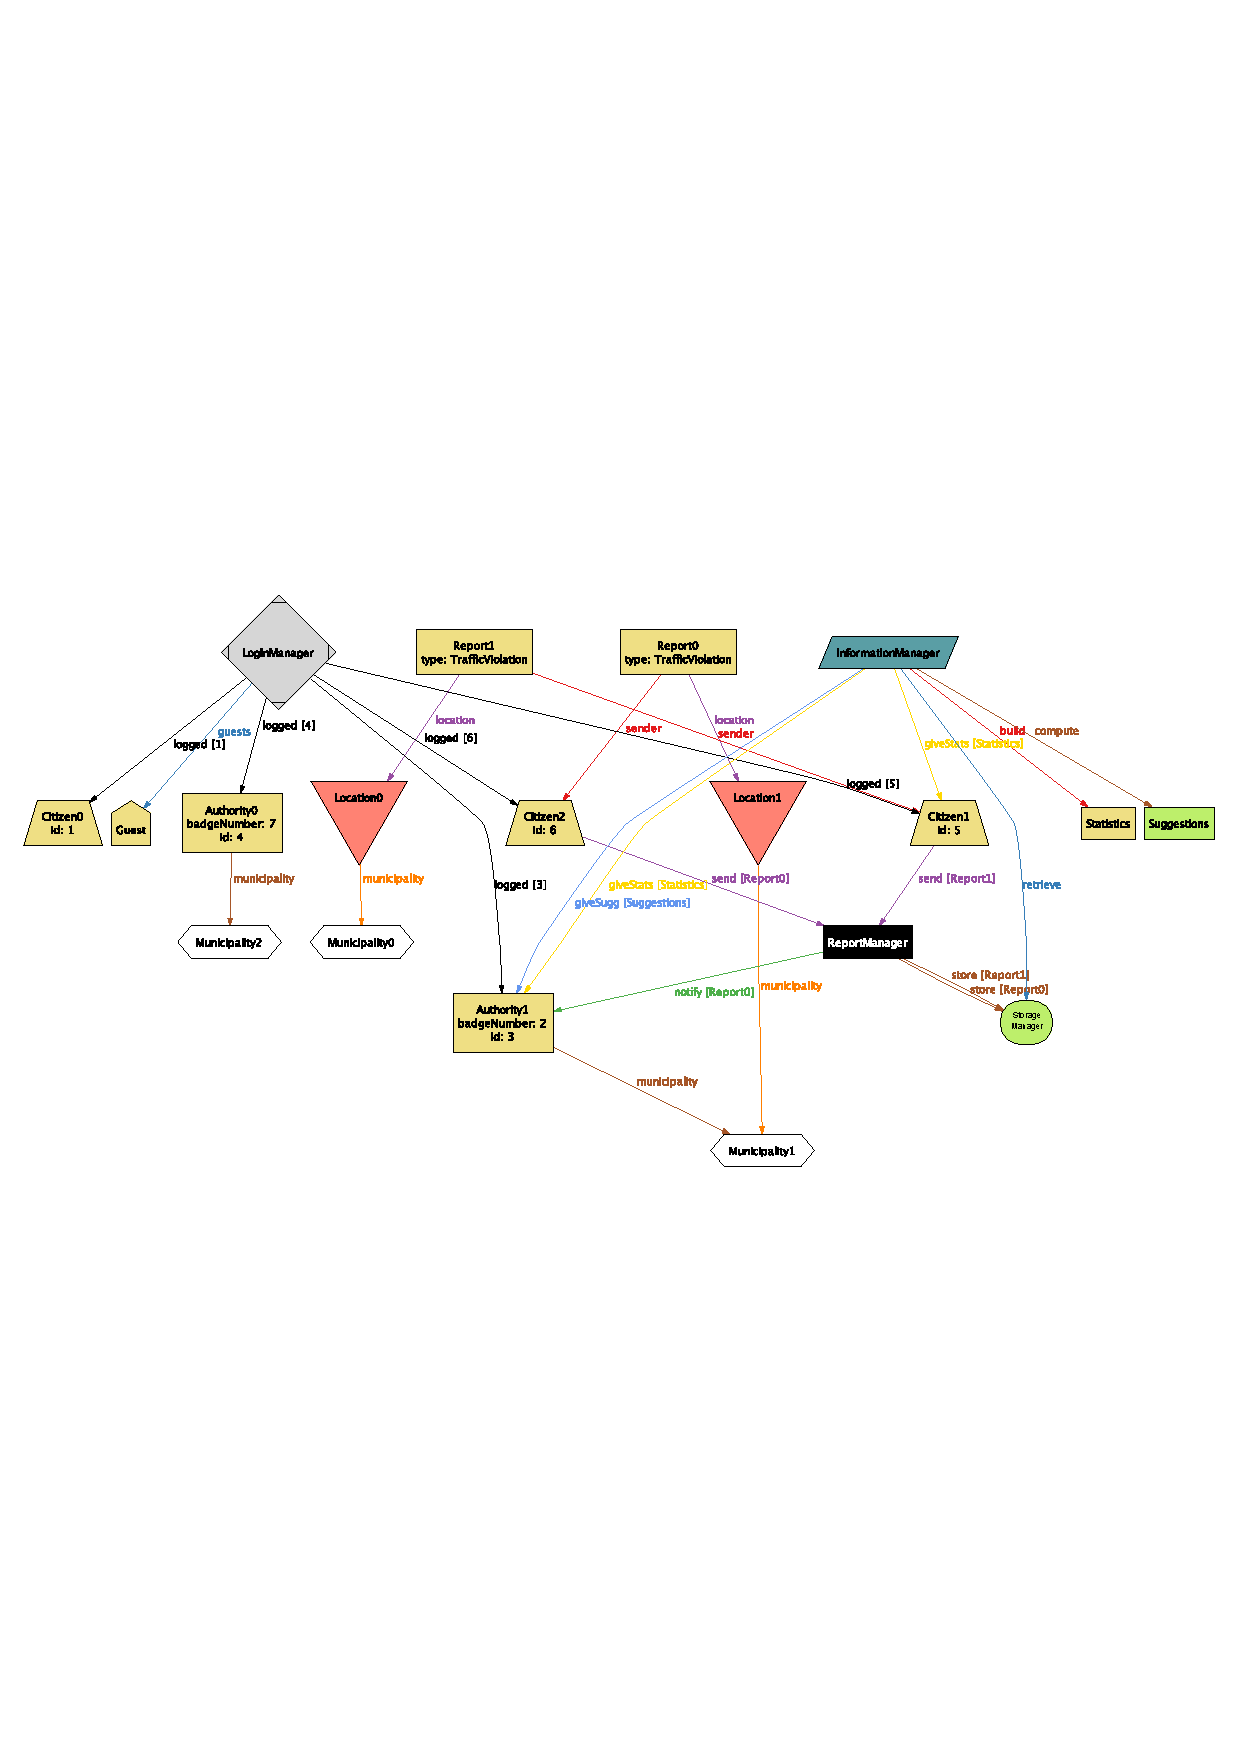
\includegraphics[width=\textwidth]{./img/Prova.pdf}
	\label{fig:all-oy}
	\caption{Alloy-generated world that shows all the possible interactions.}
	\end{center}
\end{figure}\\
In such world the Users are modeled either as Citizen or Authority, and each of them has a unique ID (and badge number, if Authority) for which the following facts hold:
\begin{lstlisting}[language=alloy]
	-- All IDs and badges are unique, different and positive integers --
	fact idsAndBadgesDifferent{
		all disj u1,u2:User | u1.id!=u2.id 
		all disj a1,a2:Authority | a1.badgeNumber!=a2.badgeNumber 
		all u1:User, a1:Authority | (u1.id!=a1.badgeNumber) and (a1.id!=a1.badgeNumber)
	}
	fact positiveId{
		all i:Int, u:User | (u.id = i implies i > 0) and (u.badgeNumber != none implies u.badgeNumber > 0)
	}
\end{lstlisting}

\subsection{Login Manager}
The Login Manager is in charge of providing the login functionality, as well as keeping a list of all the Users and the Guests who wants to log in to the application. In the Figure \ref{fig:allogin} it is shown the result of a login procedure: the Guest who requested the login in gets disconnected from the Login Manager and a new User makes its appearance in the set of the logged Users. The login manager also has to provide an ID to the new User, which has to be different from all the IDs and the badge numbers already existent.
\begin{figure}[ht!]
	\begin{center}
	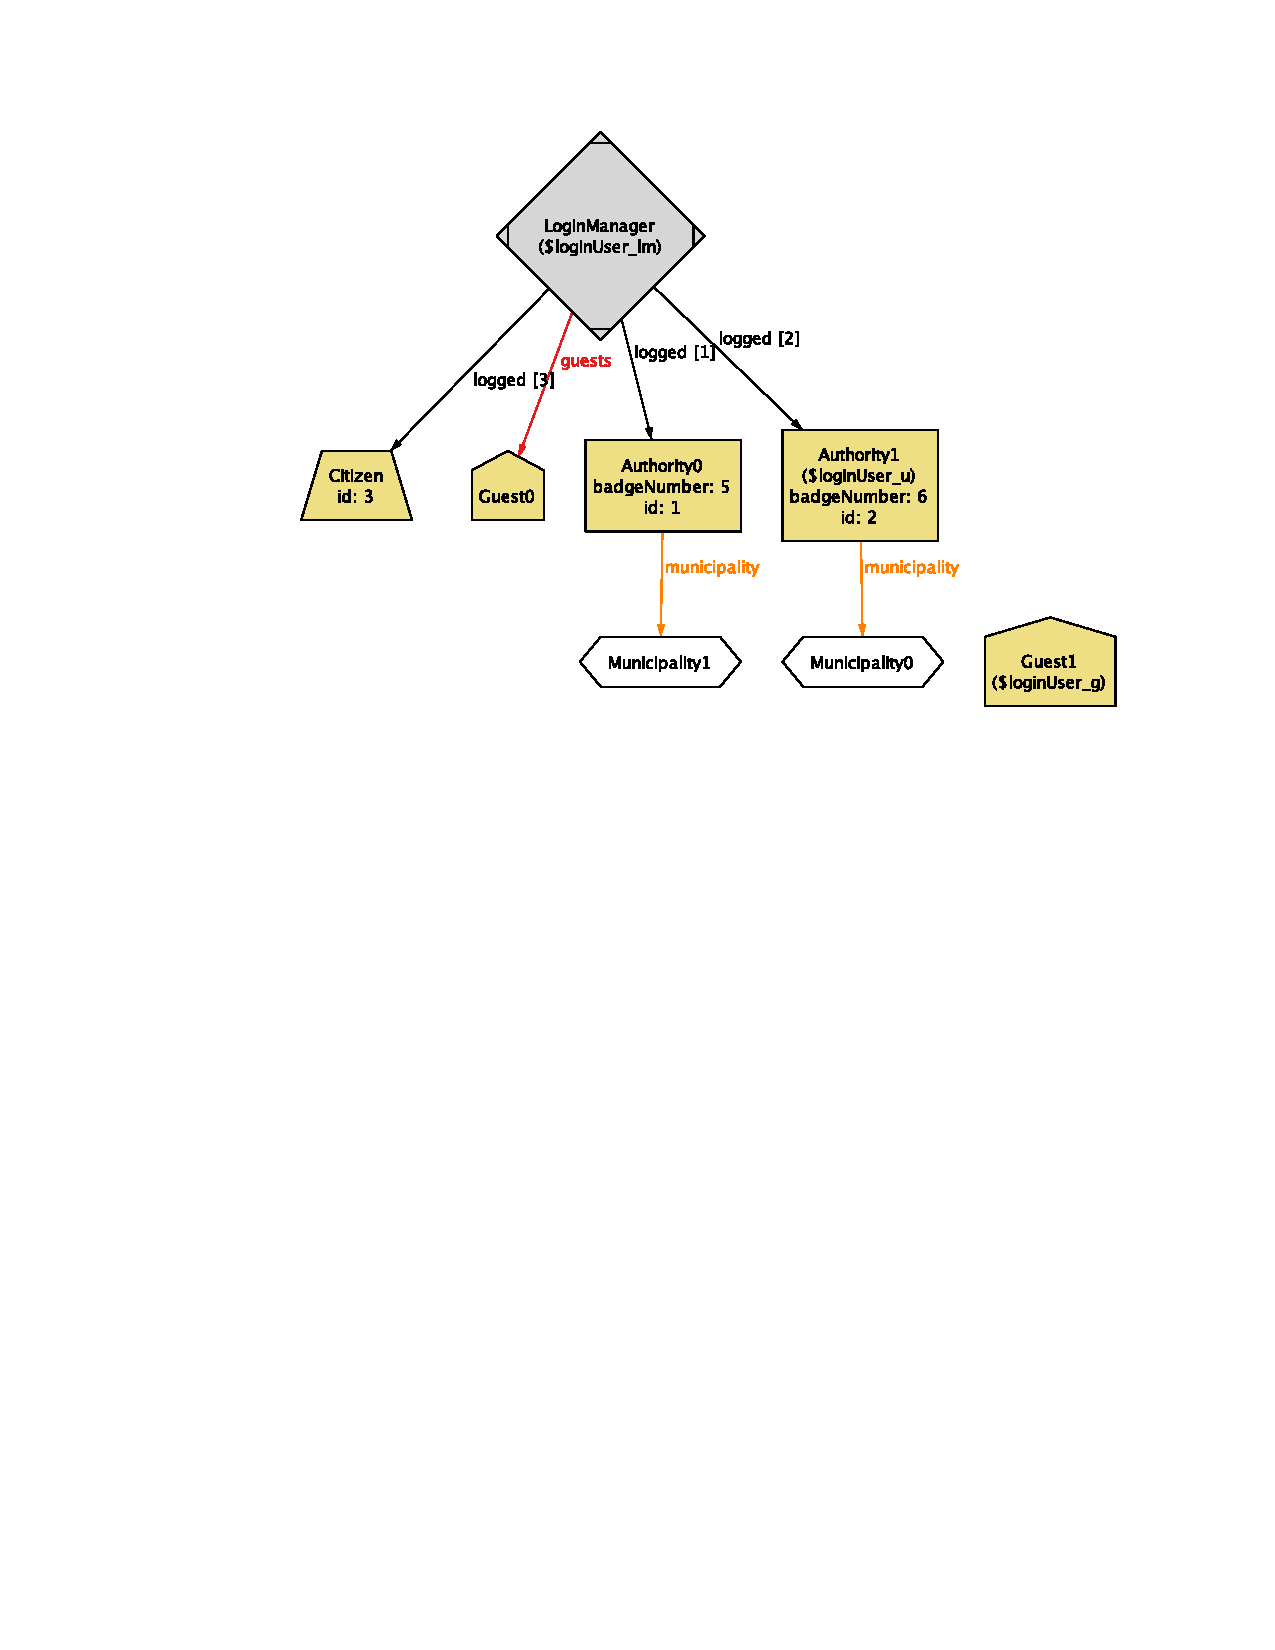
\includegraphics[width=.7\textwidth]{./img/Login.pdf}
	\label{fig:allogin}
	\caption{Alloy-generated world that shows how the login works.}
	\end{center}
\end{figure}\\
Below is the predicate which led to the Figure \ref{fig:allogin} and all the facts involved:
\begin{lstlisting}[language=alloy]
	-- Predicates used for the login procedure --
	pred disconnectedGuest{
		one g:Guest | one  lm:LoginManager | !(g in lm.guests)
	}
	pred loginUser[g:Guest, u:User, id:Int, lm:LoginManager]{
		disconnectedGuest
		lm.logged = lm.logged + (id -> u) 
	}

	-- Login Manager keeps track of all Users and Guests (except the one who logs in) --
	fact allUsersInLM{
		lone g:Guest | one  lm:LoginManager | !(g in lm.guests)
		no u:User| one lm:LoginManager | !u.id -> u in lm.logged
		all c:Citizen | (#LoginManager = 0 and #ReportManager = 1) implies #c.send > 0
		#LoginManager = 0 implies #Guest = 0
	}	
	-- Each logged User is linked to a unique integer (which is his ID) --
	fact singleId{
		no disj i1,i2:Int, u:User, lm:LoginManager | i1->u in lm.logged and i2->u in lm.logged 
	}

	run loginUser for 6 but 4 Int
\end{lstlisting}
\subsection{Report Manager}
The Report Manager's job is to collect all the Reports send by the Users, store them into the database, and notify the Authorities of the same Municipality in which the violation took place. As previously mentioned, unlike the other violations, accidents are not notified to Authorities.
\begin{figure}[ht!]
	\begin{center}
	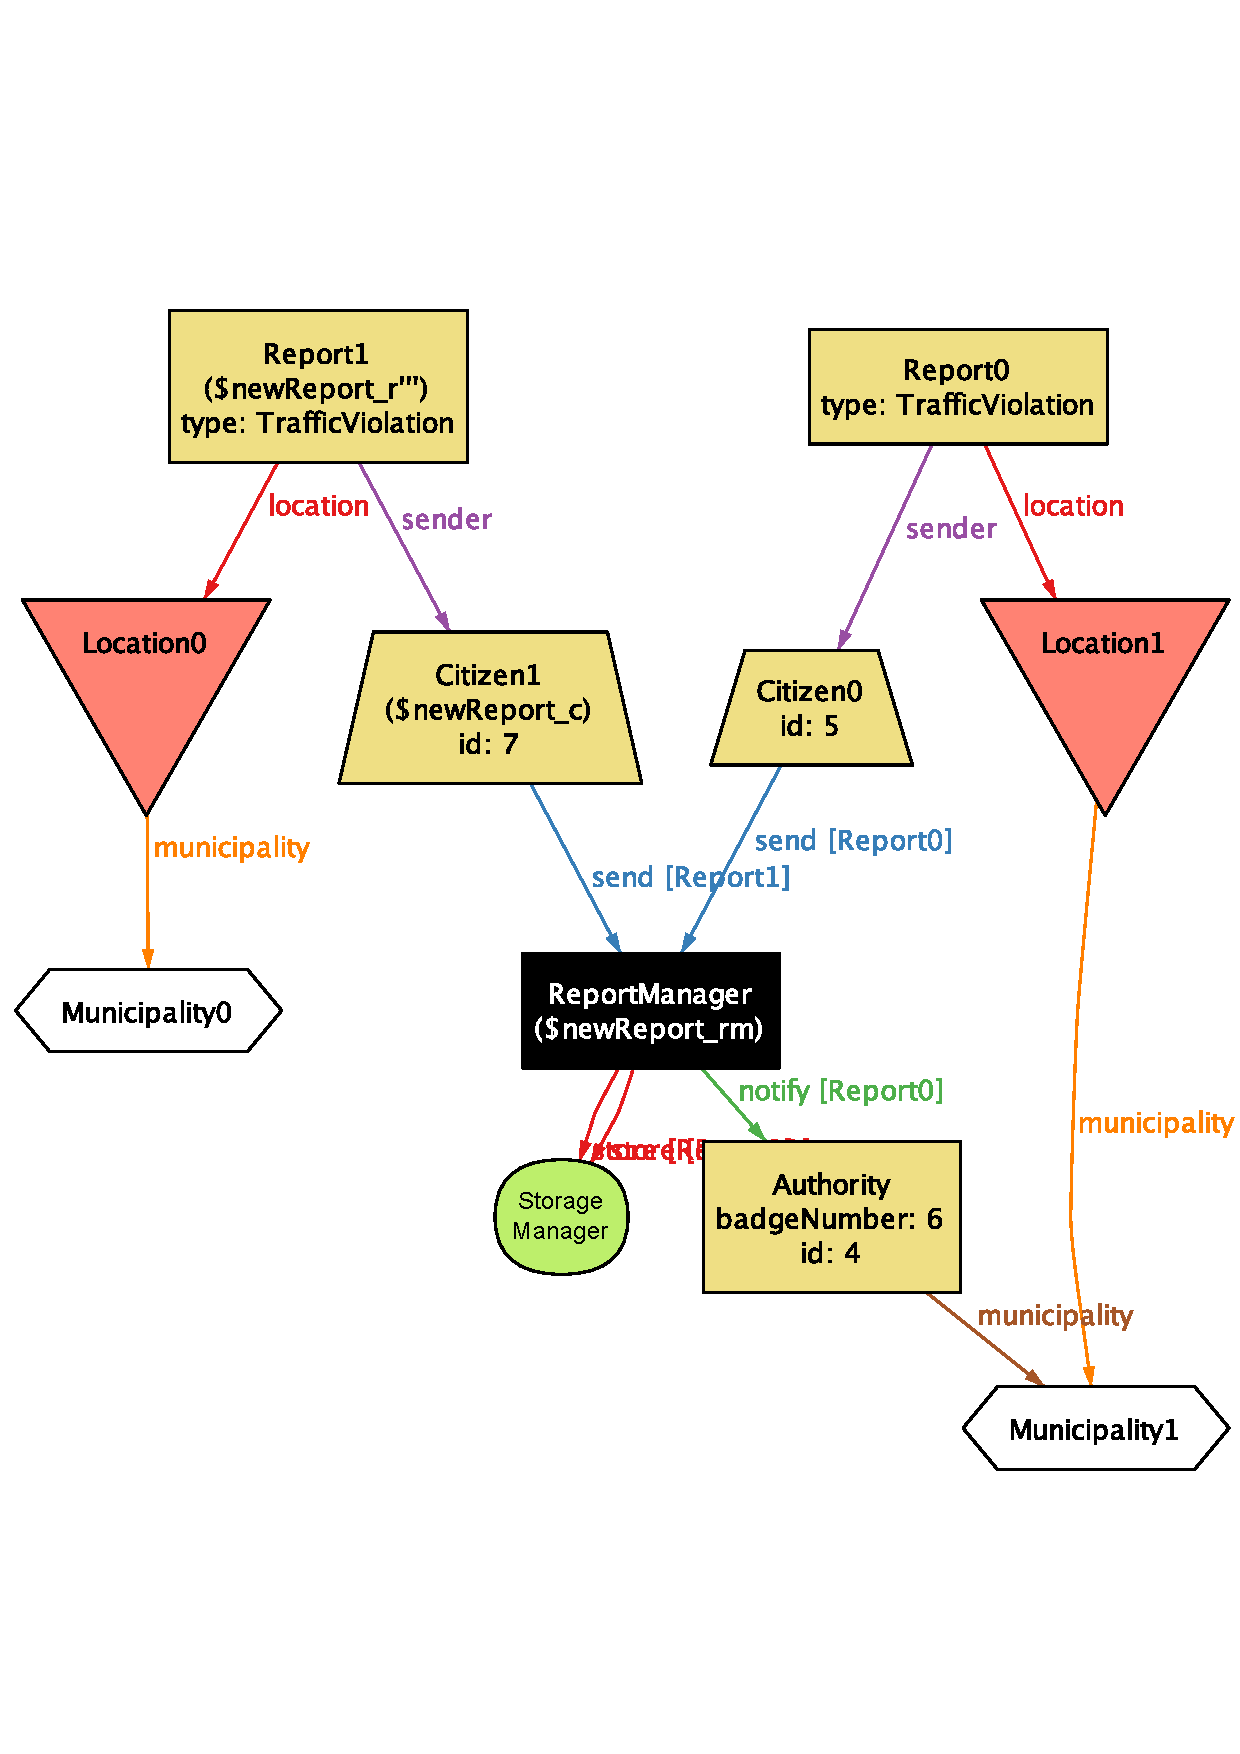
\includegraphics[width=.7\textwidth]{./img/NewReport.pdf}
	\label{fig:alloyreport}
	\caption{Alloy-generated world that shows what happens when a new report is submitted.}
	\end{center}
\end{figure}\\
Here are shown all the facts that involve Reports, as well as the predicate which generates a new one:\vfill
\begin{lstlisting}[language=alloy]
	-- Predicate used to add a new Report --
	pred newReport[r:Report, c:Citizen, rm:ReportManager]{
		!disconnectedGuest
		c.send=c.send + (r -> rm)
	}
	-- All reports are sent to the RM and then stored --
	fact reportSend{
		all r:Report, c:Citizen |one rm:ReportManager | (r.sender=c) <=>( r->rm in c.send)
	}
	fact reportStore{
		all rm:ReportManager, r:Report |one db:DBMS | r->db in rm.store
	}
	-- The Report Manager notifies Authorities with only traffic violations that involve their municipality --
		fact notifyReportBasedOnTypeAndMunicipality{
		all a:Authority,r:Report |one rm:ReportManager | ((r.type = TrafficViolation) and (r.location.municipality =a.municipality)) <=> (r->a in rm.notify) 
	}
	-- All municipalities must be involved in a violation or are supervised by at least an Authority --
	fact noReportNoMunicipality{
		all m:Municipality | (some r:Report | getMunicipality[r] = m ) or (some a:Authority | a.municipality = m )	
		no l:Location | (no r:Report | l = r.location)
	}
	-- Violations and Accidents exists only if reported --
	fact noTypesWithoutReport{
		no v:TrafficViolation| ( no r: Report | r.type = v)
		no i:Incident| ( no r: Report | r.type = i)	
	}

	run newReport for 6 but 4 Int
\end{lstlisting}
\subsection{Information Manager}
The Information manager retrives from the Storage Manager the information it needs, it builds statistics, computes suggestions, and makes them all available to the Users. Only Authorities have the permission to see safety suggestions, as they are the ones who are supposed to apply them.\vfill
\begin{figure}[ht!]
	\begin{center}
	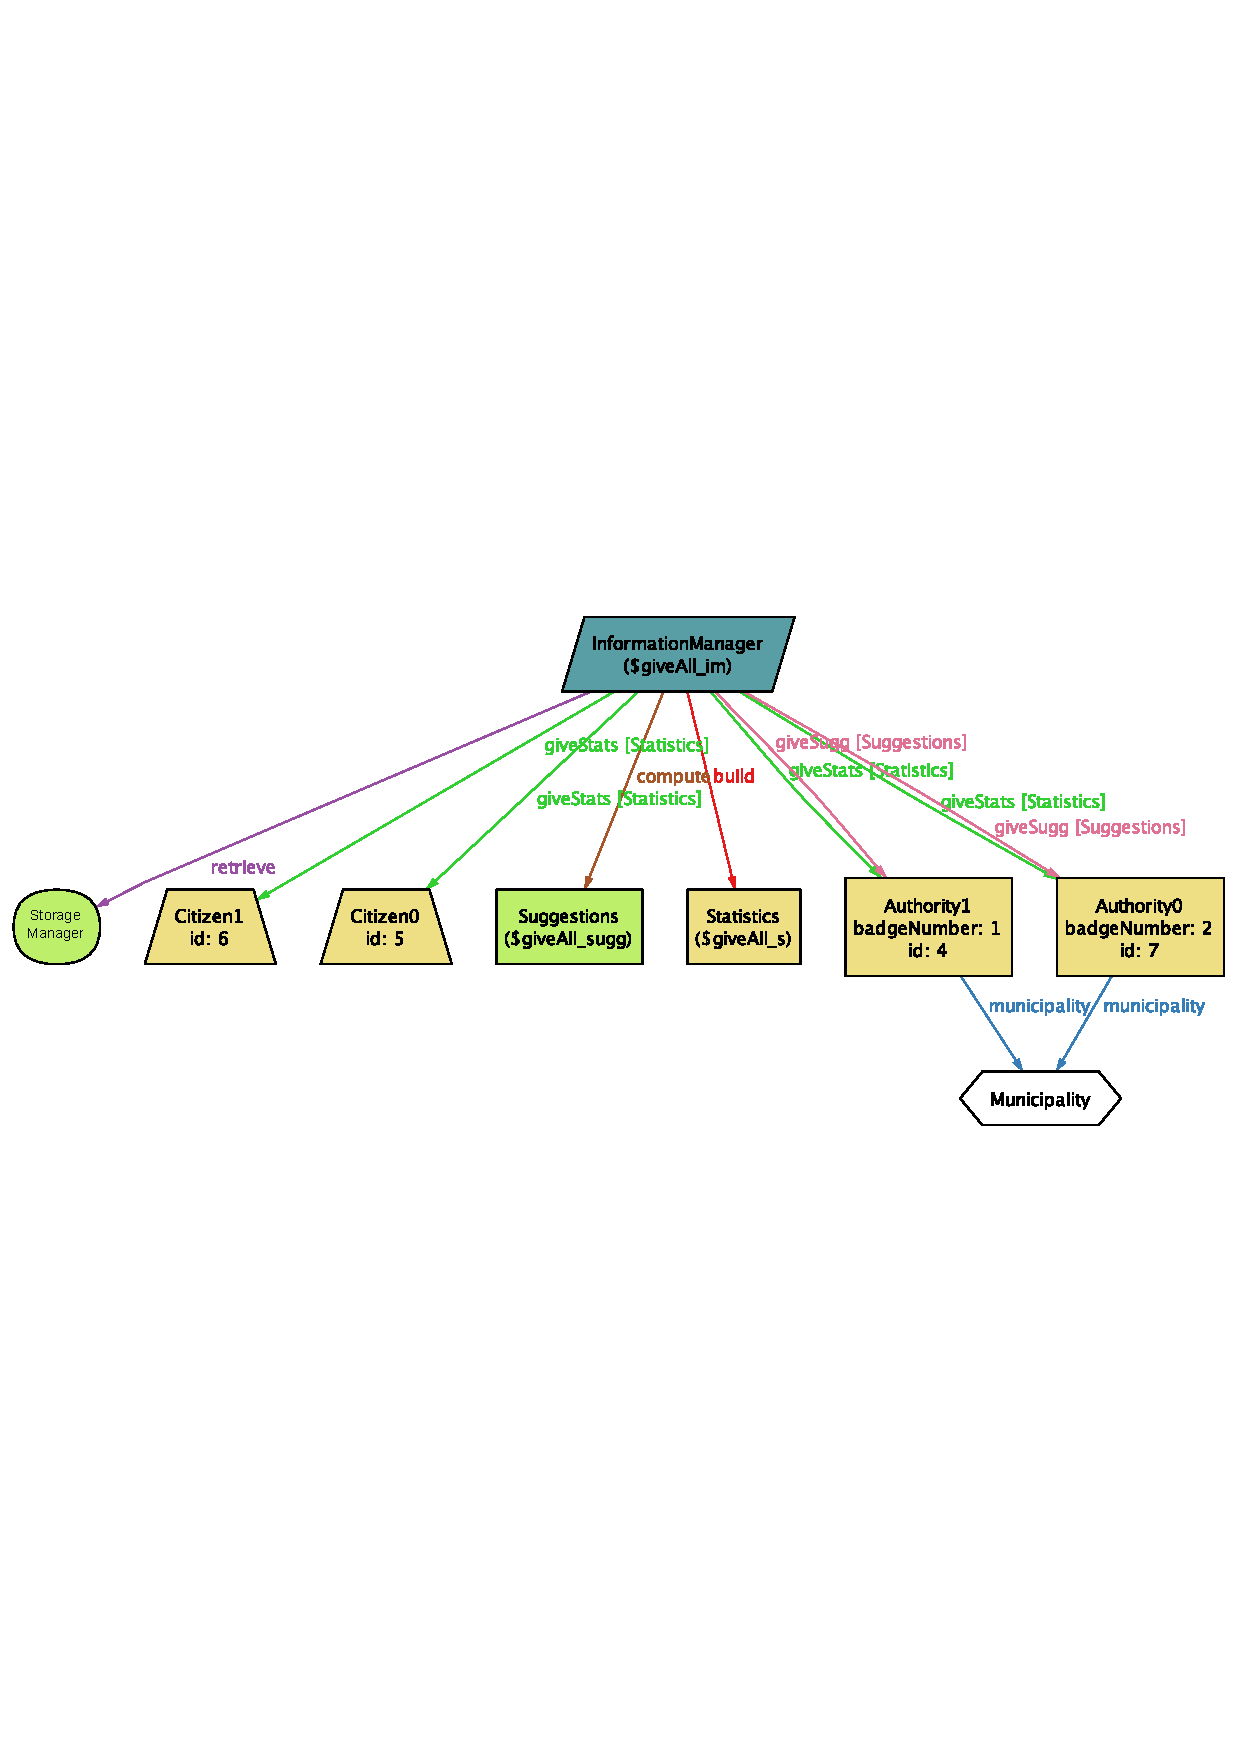
\includegraphics[width=.8\textwidth]{./img/giveAll.pdf}
	\label{fig:allgive}
	\caption{Alloy-generated world that shows how the statistics and suggestions are distributed.}
	\end{center}
\end{figure}
\noindent Here are shown the facts involving statistics, suggestions and the predicates that makes them available to the Users:
\begin{lstlisting}[language=alloy]
	-- Predicate used to give Suggestions and Statistics --
	pred giveStatistics[u:User, im:InformationManager, s:Statistics, sugg:Suggestions]{
		im.giveStats = im.giveStats + (s -> u)
	}
	pred giveAll[s:Statistics, sugg:Suggestions, im:InformationManager]{
		all u:User | giveStatistics[u, im, s, sugg]
	}
	-- Statistics and Suggestions are only generated by the Information Manager --
	fact noInfoManagerNoStatistics{
		all s:Statistics| one i:InformationManager | s in i.build 
		all s:Suggestions| one i:InformationManager | s in i.compute
	}
	-- Visibility constraints --
	fact giveStatsAndSuggs{
		all u:User, im:InformationManager | (im.build != none) implies (im.build -> u in im.giveStats)
		all im:InformationManager, u:User, s:Statistics, su: Suggestions | (u.badgeNumber != none and s->u in im.giveStats) <=> (su -> u in im.giveSugg)
		no c:Citizen, s:Suggestions, im:InformationManager | s->c in im.giveSugg
	}

	run giveAll for 6 but 4 Int
\end{lstlisting}
\section{Model Check}
\begin{lstlisting}[language=alloy]
	assert allDifferendIdsBadges{
	no disj u1,u2:User| (u1.id = u2.id) or (u2.badgeNumber != none and u1.id = u2.badgeNumber) or (u1.badgeNumber != none and u2.badgeNumber != none and  u1.badgeNumber = u2.badgeNumber)
	}
	assert oneMunicipalityOneAuthority{
		no disj m1,m2:Municipality, a:Authority | a.municipality=m1 and a.municipality=m2
	}
	assert writerReportDifferent{
		no disj c1,c2:Citizen, r:Report | r.sender=c1 and r.sender=c2
	}
	assert allReportHasWriter{
		no r:Report | no c:Citizen | r.sender = c
	}
	assert notifyReportBasedOnMunicipality{
		no r :Report, a: Authority, rm: ReportManager | (r->a in rm.notify) and (r.location.municipality != a.municipality) 
	}
	assert notifyReportBasedOnType{
		no r :Report, a: Authority, rm: ReportManager | (r->a in rm.notify) and (r.type = Incident) 
	}
	assert suggestionsVisibility{
		no c:Citizen, im:InformationManager |(im.compute != none) and (im.compute -> c in im.giveSugg)
	}
	assert allUsersCanSeeStatistics{
		no u:User, im:InformationManager | (im.build != none) and !(im.build -> u in im.giveStats)
	}
	assert noWanderingClient{
		all c:Client | all r:Report, im:InformationManager, lm:LoginManager| (r.sender = c) or (c in lm.guests or c.id->c in lm.logged) or (im.build ->c in im.giveStats) or (c.municipality != none)
	} 
	assert allUsersLoggedWithID{
		no u:User, lm:LoginManager, i:Int | (i->u in lm.logged) and (i != u.id)
	}
	assert onlyRMandIMaccessDBMS{
		no d:DBMS, rm:ReportManager, im:InformationManager | rm = none and im = none and d != none
	}
\end{lstlisting}
\begin{figure}[ht!]
    \centering
    \begin{minipage}{0.45\textwidth}
        \centering
        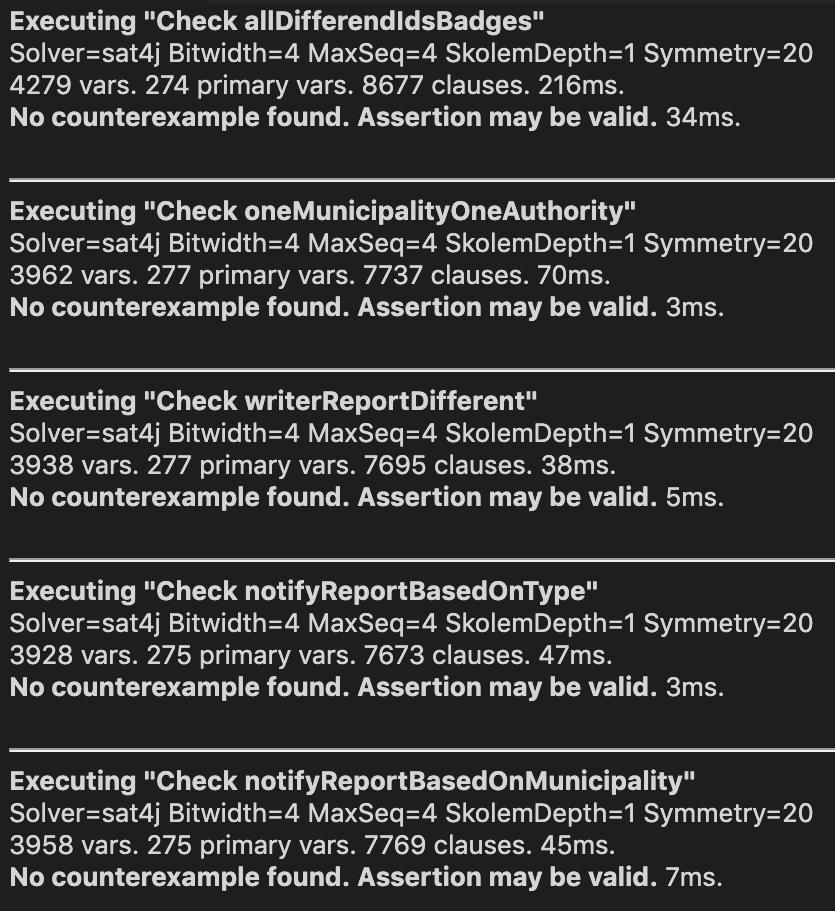
\includegraphics[width=0.9\textwidth]{./img/assert1.png} % first figure itself
    \end{minipage}\hfill
    \begin{minipage}{0.45\textwidth}
        \centering
        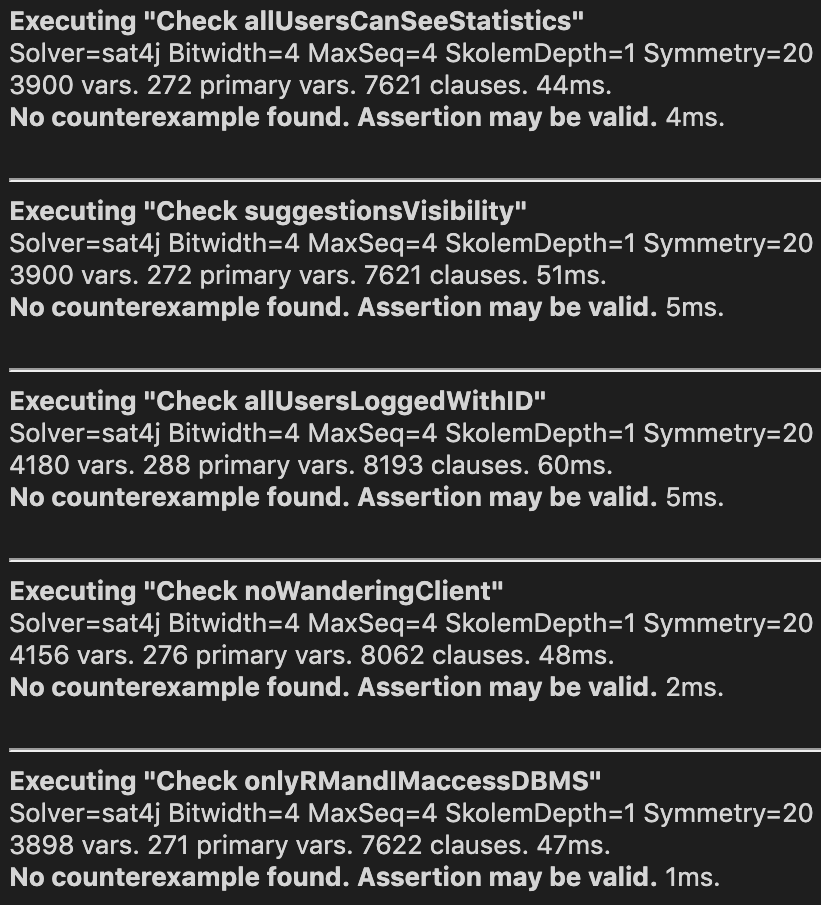
\includegraphics[width=0.9\textwidth]{./img/assert2.png} % second figure itself
	\end{minipage}
	\label{fig:modelcheck}
	\caption{Results for running all the assertions above. No counterexample is found.}
\end{figure}
\newpage
\section{Whole Alloy Model}
\begin{lstlisting}[language=alloy]

	-- SIGNATURES -- 
	abstract sig ReportType{}
	lone abstract sig Incident extends ReportType{}
	lone abstract sig TrafficViolation extends ReportType{}
	lone sig Statistics{}
	lone sig Suggestions{}
	lone sig DBMS{}
	
	sig Municipality{}
	sig Location{
		municipality: one Municipality
	}
	
	abstract sig Client {}
	sig Guest extends Client {}
	abstract sig User extends Client {
		id: one Int
	}
	sig Citizen extends User {
		send: Report -> ReportManager 
	}
	sig Authority extends User {
		badgeNumber: one Int,
		municipality: one Municipality
	}
	
	sig Report {
		type: one ReportType,
		location: one Location,
		sender: one Citizen,
	}
	
	lone sig ReportManager{
		notify: Report-> Authority,
		store: Report -> DBMS
	}
	lone sig InformationManager{
		retrieve: DBMS,
		build: lone Statistics,
		compute: lone Suggestions,
		giveStats: Statistics -> User,
		giveSugg: Suggestions -> User
	}
	lone sig LoginManager{
		guests : set Guest,
		logged : Int -> User
	}
	
	-- FUNCTIONS -- 
	fun getMunicipality[r:Report] : Municipality{
		r.(location.municipality)
	}
	
	-- FACTS -- 
	fact reportSend{
		all r:Report, c:Citizen |one rm:ReportManager | (r.sender=c) <=>( r->rm in c.send)
	}
	fact reportStore{
		all rm:ReportManager, r:Report |one db:DBMS | r->db in rm.store
	}
	fact notifyReportBasedOnTypeAndMunicipality{
		all a:Authority,r:Report |one rm:ReportManager | ((r.type = TrafficViolation) and (r.location.municipality =a.municipality)) <=> (r->a in rm.notify) 
	}
	fact idsAndBadgesDifferent{
		all disj u1,u2:User | u1.id!=u2.id 
		all disj a1,a2:Authority | a1.badgeNumber!=a2.badgeNumber 
		all u1:User, a1:Authority | (u1.id!=a1.badgeNumber) and (a1.id!=a1.badgeNumber)
	}
	fact noReportNoMunicipality{
		all m:Municipality | (some r:Report | getMunicipality[r] = m ) or (some a:Authority | a.municipality = m )	
		no l:Location | (no r:Report | l = r.location)
	}
	fact noInfoManagerNoStatistics{
		all s:Statistics| one i:InformationManager | s in i.build 
		all s:Suggestions| one i:InformationManager | s in i.compute
	}
	fact giveStatsAndSuggs{
		all u:User, im:InformationManager | (im.build != none) implies (im.build -> u in im.giveStats)
		all im:InformationManager, u:User, s:Statistics, su: Suggestions | (u.badgeNumber != none and s->u in im.giveStats) <=> (su -> u in im.giveSugg)
		no c:Citizen, s:Suggestions, im:InformationManager | s->c in im.giveSugg
	}
	fact allUsersInLM{
		lone g:Guest | one  lm:LoginManager | !(g in lm.guests)
		no u:User| one lm:LoginManager | !u.id -> u in lm.logged
		all c:Citizen | (#LoginManager = 0 and #ReportManager = 1) implies #c.send > 0
		#LoginManager = 0 implies #Guest = 0

	}
	fact positiveId{
		all i:Int, u:User | (u.id = i implies i > 0) and (u.badgeNumber != none implies u.badgeNumber > 0)
		all i:Int, u:User, lm:LoginManager |  i->u in lm.logged implies i>0 
	}
	fact singleId{
		no disj i1,i2:Int, u:User, lm:LoginManager | i1->u in lm.logged and i2->u in lm.logged 
	}
	fact noTypesWithoutReport{
		no v:TrafficViolation| ( no r: Report | r.type = v)
		no i:Incident| ( no r: Report | r.type = i)	
	}
	fact aloneDBMS{
		(#InformationManager = 0 and #ReportManager = 0) implies #DBMS = 0
	}
	
	-- ASSERTIONS -- 
	assert allDifferendIdsBadges{
	no disj u1,u2:User| (u1.id = u2.id) or (u2.badgeNumber != none and u1.id = u2.badgeNumber) or (u1.badgeNumber != none and u2.badgeNumber != none and  u1.badgeNumber = u2.badgeNumber)
	}
	assert oneMunicipalityOneAuthority{
		no disj m1,m2:Municipality, a:Authority | a.municipality=m1 and a.municipality=m2
	}
	assert writerReportDifferent{
		no disj c1,c2:Citizen, r:Report | r.sender=c1 and r.sender=c2
	}
	assert allReportHasWriter{
		no r:Report | no c:Citizen | r.sender = c
	}
	assert notifyReportBasedOnMunicipality{
		no r :Report, a: Authority, rm: ReportManager | (r->a in rm.notify) and (r.location.municipality != a.municipality) 
	}
	assert notifyReportBasedOnType{
		no r :Report, a: Authority, rm: ReportManager | (r->a in rm.notify) and (r.type = Incident) 
	}
	assert suggestionsVisibility{
		no c:Citizen, im:InformationManager |(im.compute != none) and (im.compute -> c in im.giveSugg)
	}
	assert allUsersCanSeeStatistics{
		no u:User, im:InformationManager | (im.build != none) and !(im.build -> u in im.giveStats)
	}
	assert noWanderingClient{
		all c:Client | all r:Report, im:InformationManager, lm:LoginManager| (r.sender = c) or (c in lm.guests or c.id->c in lm.logged) or (im.build ->c in im.giveStats) or (c.municipality != none)
	} 
	assert allUsersLoggedWithID{
		no u:User, lm:LoginManager, i:Int | (i->u in lm.logged) and (i != u.id)
	}
	assert onlyRMandIMaccessDBMS{
		no d:DBMS, rm:ReportManager, im:InformationManager | rm = none and im = none and d != none
	}
	
	-- PREDICATES -- 
	pred newReport[r:Report, c:Citizen, rm:ReportManager]{
		!disconnectedGuest
		c.send=c.send + (r -> rm)
	}
	pred loginUser[g:Guest, u:User, id:Int, lm:LoginManager]{
		disconnectedGuest
		lm.logged = lm.logged + (id -> u) 
	}
	pred disconnectedGuest{
		one g:Guest | one  lm:LoginManager | !(g in lm.guests)
	}
	pred showUser{
		!disconnectedGuest
	}
	pred giveStatistics[u:User, im:InformationManager, s:Statistics, sugg:Suggestions]{
		im.giveStats = im.giveStats + (s -> u)
	}
	pred giveAll[s:Statistics, sugg:Suggestions, im:InformationManager]{
		all u:User | giveStatistics[u, im, s, sugg]
	}

-- EXECUTION -- 
run showUser for 6 but 4 Int
run newReport for 6 but 4 Int
run giveAll for 6 but 4 Int
run loginUser for 6 but 4 Int

	\end{lstlisting}
\chapter{Effort Spent}
\subsection*{Francesco Amorosini}
\begin{table}[!ht]
	\begin{tabular}{|C{.60\textwidth}||C{.20\textwidth}|}
		\toprule
		\textbf{Task} & \textbf{Hours}\\
		\midrule
		\midrule
		Meeting for analysis of task & 4\\
		\midrule
		Tools and Github setup for the project & 2\\
		\midrule
		Purpose and Scope & 3.5\\
		\midrule
		Product Functions& 3.5\\ 
		\midrule
		\small{\textbf{Mid-Phase Call}}: & \\
		\vspace{.2mm}
		$\bullet$ Functional requirements and Assumptions & \vspace{.2mm} 3\\
		$\bullet$ Goal Mapping on Requirements & 3\\
		\midrule
		Performance requirements & 1.5\\
		\midrule
		Design constraints & 3.5\\
		\midrule
		Software System Attributes & 1\\
		\midrule
		Alloy modeling & 2.5\\
		\midrule
		Alloy chapter & 4.5\\
		\midrule
		Images and tables polishing & 2.5\\
		\midrule
		Grammar correction and global review & 5.5\\
		\midrule
		& \textbf{Total:} 40\\
		\bottomrule
	\end{tabular}
\end{table}
\clearpage
\subsection*{Alice Casali}
\begin{table}[!ht]
	\begin{tabular}{|C{.60\textwidth}||C{.20\textwidth}|}
		\toprule
		\textbf{Task} & \textbf{Hours}\\
		\midrule
		\midrule
		Meeting for analysis of task & 4\\
		\midrule
		Tools and Github setup for the project & 2\\
		\midrule
		Goals discussion & 2\\
		\midrule
		Product Perspective & 3\\ 
		\midrule
		Statechart Diagrams & 3.5\\
		\midrule
		First approach on assumptions, dependencies and constraints & 1.5\\
		\midrule
		Functional Requirements & 3.5\\ 
		\midrule
		\small{\textbf{Mid-Phase Call}}: & \\
		\vspace{.2mm}
		$\bullet$ Functional requirements and Assumptions & \vspace{.2mm} 3\\
		$\bullet$ Goal Mapping on Requirements & 3\\
		\midrule
		Added new UseCase Templates & 2 \\
		\midrule
		Statecharts revision & 1\\
		\midrule
		External Interface Requirement & 1\\
		\midrule
		User interface with Mockup & 3.5\\
		\midrule
		Final revision & 2\\
		\midrule
		& \textbf{Total:} 35\\
		\bottomrule
	\end{tabular}
\end{table}

\begin{table}[!ht]
	\subsection*{Tommaso Fioravanti}
	\begin{tabular}{|C{.60\textwidth}||C{.20\textwidth}|}
		\toprule
		\textbf{Task} & \textbf{Hours}\\
		\midrule
		\midrule
		Meeting for analysis of task & 4\\
		\midrule
		Tools and Github setup for the project & 2\\
		\midrule
		Purpose and Scope & 2,5\\
		\midrule
		Overview, Definitions and Acronyms & 1,5\\
		\midrule
		Goal Analysis & 2\\
		\midrule
		Class Diagram & 2\\
		\midrule
		Use Case Diagrams and Template & 3,5\\
		\midrule
		Sequence Diagrams & 4\\
		\midrule
		Software System Attributes & 2 \\
		\midrule
		Functional Requirement and Assumptions review &1,5\\
		\midrule
		Alloy modeling& 5,5\\
		\midrule
		Sequence Diagrams review & 2\\
		\midrule
		Global review & 3\\
		\midrule
		Further refinements& 1,5\\ 
		\midrule
		& \textbf{Total:} 37\\
		\bottomrule
	\end{tabular}
\end{table}
\end{document}